\documentclass[1p]{elsarticle_modified}
%\bibliographystyle{elsarticle-num}

%\usepackage[colorlinks]{hyperref}
%\usepackage{abbrmath_seonhwa} %\Abb, \Ascr, \Acal ,\Abf, \Afrak
\usepackage{amsfonts}
\usepackage{amssymb}
\usepackage{amsmath}
\usepackage{amsthm}
\usepackage{scalefnt}
\usepackage{amsbsy}
\usepackage{kotex}
\usepackage{caption}
\usepackage{subfig}
\usepackage{color}
\usepackage{graphicx}
\usepackage{xcolor} %% white, black, red, green, blue, cyan, magenta, yellow
\usepackage{float}
\usepackage{setspace}
\usepackage{hyperref}

\usepackage{tikz}
\usetikzlibrary{arrows}

\usepackage{multirow}
\usepackage{array} % fixed length table
\usepackage{hhline}

%%%%%%%%%%%%%%%%%%%%%
\makeatletter
\renewcommand*\env@matrix[1][\arraystretch]{%
	\edef\arraystretch{#1}%
	\hskip -\arraycolsep
	\let\@ifnextchar\new@ifnextchar
	\array{*\c@MaxMatrixCols c}}
\makeatother %https://tex.stackexchange.com/questions/14071/how-can-i-increase-the-line-spacing-in-a-matrix
%%%%%%%%%%%%%%%

\usepackage[normalem]{ulem}

\newcommand{\msout}[1]{\ifmmode\text{\sout{\ensuremath{#1}}}\else\sout{#1}\fi}
%SOURCE: \msout is \stkout macro in https://tex.stackexchange.com/questions/20609/strikeout-in-math-mode

\newcommand{\cancel}[1]{
	\ifmmode
	{\color{red}\msout{#1}}
	\else
	{\color{red}\sout{#1}}
	\fi
}

\newcommand{\add}[1]{
	{\color{blue}\uwave{#1}}
}

\newcommand{\replace}[2]{
	\ifmmode
	{\color{red}\msout{#1}}{\color{blue}\uwave{#2}}
	\else
	{\color{red}\sout{#1}}{\color{blue}\uwave{#2}}
	\fi
}

\newcommand{\Sol}{\mathcal{S}} %segment
\newcommand{\D}{D} %diagram
\newcommand{\A}{\mathcal{A}} %arc


%%%%%%%%%%%%%%%%%%%%%%%%%%%%%5 test

\def\sl{\operatorname{\textup{SL}}(2,\Cbb)}
\def\psl{\operatorname{\textup{PSL}}(2,\Cbb)}
\def\quan{\mkern 1mu \triangleright \mkern 1mu}

\theoremstyle{definition}
\newtheorem{thm}{Theorem}[section]
\newtheorem{prop}[thm]{Proposition}
\newtheorem{lem}[thm]{Lemma}
\newtheorem{ques}[thm]{Question}
\newtheorem{cor}[thm]{Corollary}
\newtheorem{defn}[thm]{Definition}
\newtheorem{exam}[thm]{Example}
\newtheorem{rmk}[thm]{Remark}
\newtheorem{alg}[thm]{Algorithm}

\newcommand{\I}{\sqrt{-1}}
\begin{document}

%\begin{frontmatter}
%
%\title{Boundary parabolic representations of knots up to 8 crossings}
%
%%% Group authors per affiliation:
%\author{Yunhi Cho} 
%\address{Department of Mathematics, University of Seoul, Seoul, Korea}
%\ead{yhcho@uos.ac.kr}
%
%
%\author{Seonhwa Kim} %\fnref{s_kim}}
%\address{Center for Geometry and Physics, Institute for Basic Science, Pohang, 37673, Korea}
%\ead{ryeona17@ibs.re.kr}
%
%\author{Hyuk Kim}
%\address{Department of Mathematical Sciences, Seoul National University, Seoul 08826, Korea}
%\ead{hyukkim@snu.ac.kr}
%
%\author{Seokbeom Yoon}
%\address{Department of Mathematical Sciences, Seoul National University, Seoul, 08826,  Korea}
%\ead{sbyoon15@snu.ac.kr}
%
%\begin{abstract}
%We find all boundary parabolic representation of knots up to 8 crossings.
%
%\end{abstract}
%\begin{keyword}
%    \MSC[2010] 57M25 
%\end{keyword}
%
%\end{frontmatter}

%\linenumbers
%\tableofcontents
%
\newcommand\colored[1]{\textcolor{white}{\rule[-0.35ex]{0.8em}{1.4ex}}\kern-0.8em\color{red} #1}%
%\newcommand\colored[1]{\textcolor{white}{ #1}\kern-2.17ex	\textcolor{white}{ #1}\kern-1.81ex	\textcolor{white}{ #1}\kern-2.15ex\color{red}#1	}

{\Large $\underline{12a_{1155}~(K12a_{1155})}$}

\setlength{\tabcolsep}{10pt}
\renewcommand{\arraystretch}{1.6}
\vspace{1cm}\begin{tabular}{m{100pt}>{\centering\arraybackslash}m{274pt}}
\multirow{5}{120pt}{
	\centering
	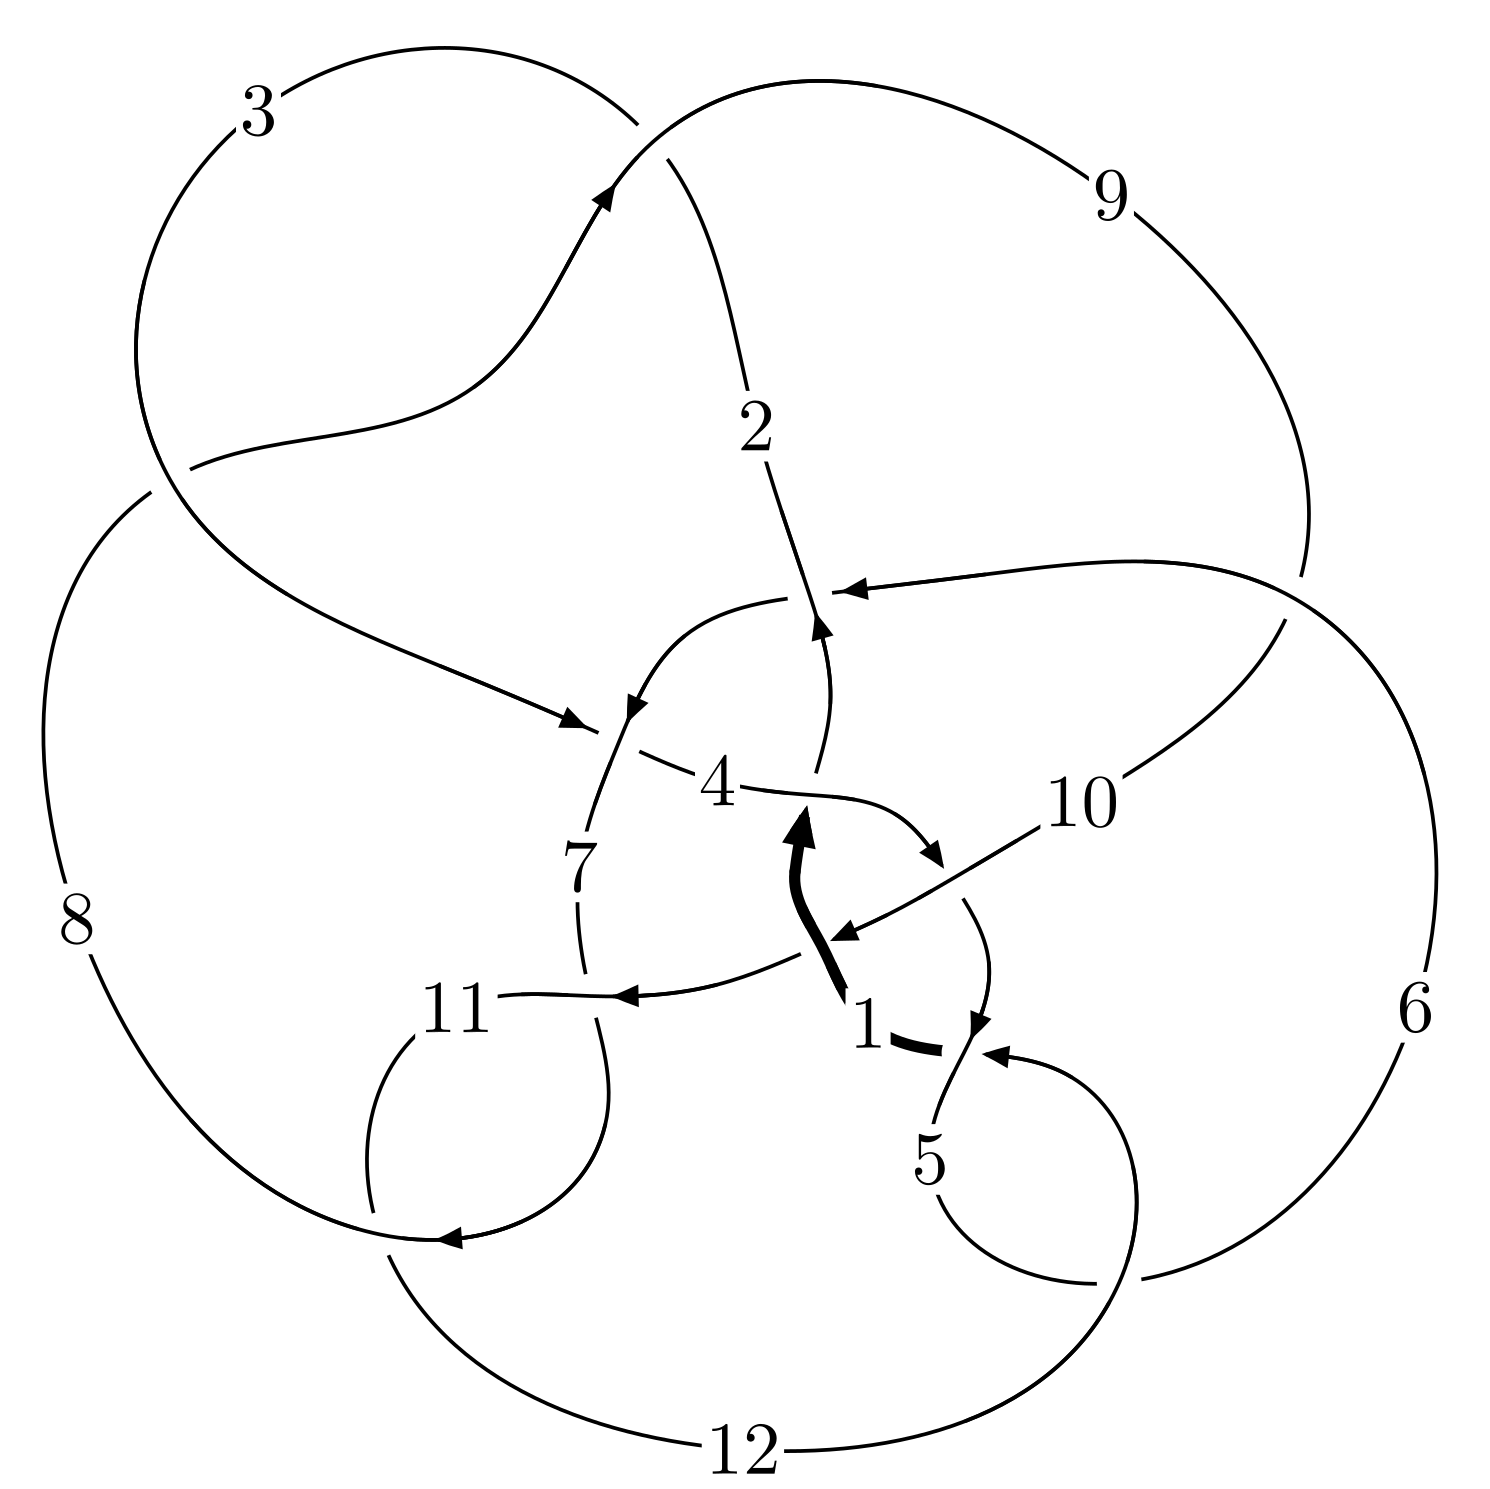
\includegraphics[width=112pt]{../../../GIT/diagram.site/Diagrams/png/1956_12a_1155.png}\\
\ \ \ A knot diagram\footnotemark}&
\allowdisplaybreaks
\textbf{Linearized knot diagam} \\
\cline{2-2}
 &
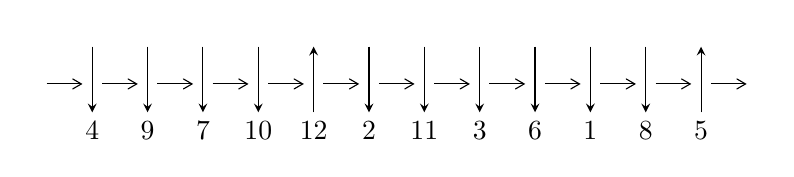
\begin{tikzpicture}[x=20pt, y=17pt]
	% nodes
	\node (C0) at (0, 0) {};
	\node (C1) at (1, 0) {};
	\node (C1U) at (1, +1) {};
	\node (C1D) at (1, -1) {4};

	\node (C2) at (2, 0) {};
	\node (C2U) at (2, +1) {};
	\node (C2D) at (2, -1) {9};

	\node (C3) at (3, 0) {};
	\node (C3U) at (3, +1) {};
	\node (C3D) at (3, -1) {7};

	\node (C4) at (4, 0) {};
	\node (C4U) at (4, +1) {};
	\node (C4D) at (4, -1) {10};

	\node (C5) at (5, 0) {};
	\node (C5U) at (5, +1) {};
	\node (C5D) at (5, -1) {12};

	\node (C6) at (6, 0) {};
	\node (C6U) at (6, +1) {};
	\node (C6D) at (6, -1) {2};

	\node (C7) at (7, 0) {};
	\node (C7U) at (7, +1) {};
	\node (C7D) at (7, -1) {11};

	\node (C8) at (8, 0) {};
	\node (C8U) at (8, +1) {};
	\node (C8D) at (8, -1) {3};

	\node (C9) at (9, 0) {};
	\node (C9U) at (9, +1) {};
	\node (C9D) at (9, -1) {6};

	\node (C10) at (10, 0) {};
	\node (C10U) at (10, +1) {};
	\node (C10D) at (10, -1) {1};

	\node (C11) at (11, 0) {};
	\node (C11U) at (11, +1) {};
	\node (C11D) at (11, -1) {8};

	\node (C12) at (12, 0) {};
	\node (C12U) at (12, +1) {};
	\node (C12D) at (12, -1) {5};
	\node (C13) at (13, 0) {};

	% arrows
	\draw[->,>={angle 60}]
	(C0) edge (C1) (C1) edge (C2) (C2) edge (C3) (C3) edge (C4) (C4) edge (C5) (C5) edge (C6) (C6) edge (C7) (C7) edge (C8) (C8) edge (C9) (C9) edge (C10) (C10) edge (C11) (C11) edge (C12) (C12) edge (C13) ;	\draw[->,>=stealth]
	(C1U) edge (C1D) (C2U) edge (C2D) (C3U) edge (C3D) (C4U) edge (C4D) (C5D) edge (C5U) (C6U) edge (C6D) (C7U) edge (C7D) (C8U) edge (C8D) (C9U) edge (C9D) (C10U) edge (C10D) (C11U) edge (C11D) (C12D) edge (C12U) ;
	\end{tikzpicture} \\
\hhline{~~} \\& 
\textbf{Solving Sequence} \\ \cline{2-2} 
 &
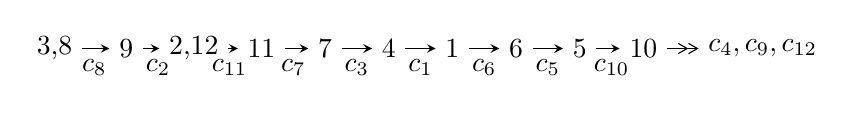
\begin{tikzpicture}[x=23pt, y=7pt]
	% node
	\node (A0) at (-1/8, 0) {3,8};
	\node (A1) at (1, 0) {9};
	\node (A2) at (33/16, 0) {2,12};
	\node (A3) at (25/8, 0) {11};
	\node (A4) at (33/8, 0) {7};
	\node (A5) at (41/8, 0) {4};
	\node (A6) at (49/8, 0) {1};
	\node (A7) at (57/8, 0) {6};
	\node (A8) at (65/8, 0) {5};
	\node (A9) at (73/8, 0) {10};
	\node (C1) at (1/2, -1) {$c_{8}$};
	\node (C2) at (3/2, -1) {$c_{2}$};
	\node (C3) at (21/8, -1) {$c_{11}$};
	\node (C4) at (29/8, -1) {$c_{7}$};
	\node (C5) at (37/8, -1) {$c_{3}$};
	\node (C6) at (45/8, -1) {$c_{1}$};
	\node (C7) at (53/8, -1) {$c_{6}$};
	\node (C8) at (61/8, -1) {$c_{5}$};
	\node (C9) at (69/8, -1) {$c_{10}$};
	\node (A10) at (11, 0) {$c_{4},c_{9},c_{12}$};

	% edge
	\draw[->,>=stealth]	
	(A0) edge (A1) (A1) edge (A2) (A2) edge (A3) (A3) edge (A4) (A4) edge (A5) (A5) edge (A6) (A6) edge (A7) (A7) edge (A8) (A8) edge (A9) ;
	\draw[->>,>={angle 60}]	
	(A9) edge (A10);
\end{tikzpicture} \\ 

\end{tabular} \\

\footnotetext{
The image of knot diagram is generated by the software ``\textbf{Draw programme}" developed by Andrew Bartholomew(\url{http://www.layer8.co.uk/maths/draw/index.htm\#Running-draw}), where we modified some parts for our purpose(\url{https://github.com/CATsTAILs/LinksPainter}).
}\phantom \\ \newline 
\centering \textbf{Ideals for irreducible components\footnotemark of $X_{\text{par}}$} 
 
\begin{align*}
I^u_{1}&=\langle 
-1.50988\times10^{1377} u^{193}+5.90345\times10^{1378} u^{192}+\cdots+5.92791\times10^{1378} b-5.34232\times10^{1384},\\
\phantom{I^u_{1}}&\phantom{= \langle  }-5.91310\times10^{1384} u^{193}-1.11374\times10^{1385} u^{192}+\cdots+4.68861\times10^{1384} a+5.14788\times10^{1390},\\
\phantom{I^u_{1}}&\phantom{= \langle  }u^{194}+u^{193}+\cdots-1651839 u-790939\rangle \\
I^u_{2}&=\langle 
-1.99760\times10^{82} u^{57}+5.15828\times10^{81} u^{56}+\cdots+1.43336\times10^{82} b-1.65100\times10^{82},\\
\phantom{I^u_{2}}&\phantom{= \langle  }1.86247\times10^{82} u^{57}+5.00930\times10^{80} u^{56}+\cdots+1.43336\times10^{82} a-3.53162\times10^{82},\;u^{58}+18 u^{56}+\cdots+u+1\rangle \\
\\
\end{align*}
\raggedright * 2 irreducible components of $\dim_{\mathbb{C}}=0$, with total 252 representations.\\
\footnotetext{All coefficients of polynomials are rational numbers. But the coefficients are sometimes approximated in decimal forms when there is not enough margin.}
\newpage
\renewcommand{\arraystretch}{1}
\centering \section*{I. $I^u_{1}= \langle -1.51\times10^{1377} u^{193}+5.90\times10^{1378} u^{192}+\cdots+5.93\times10^{1378} b-5.34\times10^{1384},\;-5.91\times10^{1384} u^{193}-1.11\times10^{1385} u^{192}+\cdots+4.69\times10^{1384} a+5.15\times10^{1390},\;u^{194}+u^{193}+\cdots-1651839 u-790939 \rangle$}
\flushleft \textbf{(i) Arc colorings}\\
\begin{tabular}{m{7pt} m{180pt} m{7pt} m{180pt} }
\flushright $a_{3}=$&$\begin{pmatrix}0\\u\end{pmatrix}$ \\
\flushright $a_{8}=$&$\begin{pmatrix}1\\0\end{pmatrix}$ \\
\flushright $a_{9}=$&$\begin{pmatrix}1\\u^2\end{pmatrix}$ \\
\flushright $a_{2}=$&$\begin{pmatrix}u\\u^3+u\end{pmatrix}$ \\
\flushright $a_{12}=$&$\begin{pmatrix}1.26116 u^{193}+2.37542 u^{192}+\cdots-3.16290\times10^{6} u-1.09795\times10^{6}\\0.0254707 u^{193}-0.995873 u^{192}+\cdots+1.73070\times10^{6} u+901215.\end{pmatrix}$ \\
\flushright $a_{11}=$&$\begin{pmatrix}1.28663 u^{193}+1.37955 u^{192}+\cdots-1.43220\times10^{6} u-196739.\\0.0254707 u^{193}-0.995873 u^{192}+\cdots+1.73070\times10^{6} u+901215.\end{pmatrix}$ \\
\flushright $a_{7}=$&$\begin{pmatrix}-0.269234 u^{193}-0.382547 u^{192}+\cdots+688122. u+201144.\\1.19256 u^{193}+1.92736 u^{192}+\cdots-2.78150\times10^{6} u-847543.\end{pmatrix}$ \\
\flushright $a_{4}=$&$\begin{pmatrix}0.579703 u^{193}+1.03632 u^{192}+\cdots-1.34421\times10^{6} u-432416.\\0.450166 u^{193}+0.872018 u^{192}+\cdots-1.27867\times10^{6} u-468981.\end{pmatrix}$ \\
\flushright $a_{1}=$&$\begin{pmatrix}0.599790 u^{193}+0.366313 u^{192}+\cdots-390711. u+57558.9\\-0.0944036 u^{193}-0.913057 u^{192}+\cdots+1.51939\times10^{6} u+741934.\end{pmatrix}$ \\
\flushright $a_{6}=$&$\begin{pmatrix}-1.43082 u^{193}-2.07265 u^{192}+\cdots+3.06205\times10^{6} u+856286.\\1.06618 u^{193}+1.57062 u^{192}+\cdots-2.19934\times10^{6} u-610425.\end{pmatrix}$ \\
\flushright $a_{5}=$&$\begin{pmatrix}-0.472776 u^{193}-0.774592 u^{192}+\cdots+1.13923\times10^{6} u+370057.\\-0.161775 u^{193}-0.0848087 u^{192}+\cdots+52404.0 u-45327.9\end{pmatrix}$ \\
\flushright $a_{10}=$&$\begin{pmatrix}1.17797 u^{193}+1.00013 u^{192}+\cdots-954147. u+24399.5\\-0.349845 u^{193}-0.676480 u^{192}+\cdots+936578. u+319712.\end{pmatrix}$\\&\end{tabular}
\flushleft \textbf{(ii) Obstruction class $= -1$}\\~\\
\flushleft \textbf{(iii) Cusp Shapes $= 3.42353 u^{193}+12.3533 u^{192}+\cdots-1.94793\times10^{7} u-8.52189\times10^{6}$}\\~\\
\newpage\renewcommand{\arraystretch}{1}
\flushleft \textbf{(iv) u-Polynomials at the component}\newline \\
\begin{tabular}{m{50pt}|m{274pt}}
Crossings & \hspace{64pt}u-Polynomials at each crossing \\
\hline $$\begin{aligned}c_{1}\end{aligned}$$&$\begin{aligned}
&u^{194}-11 u^{193}+\cdots-62880330 u+4090161
\end{aligned}$\\
\hline $$\begin{aligned}c_{2},c_{8}\end{aligned}$$&$\begin{aligned}
&u^{194}- u^{193}+\cdots+1651839 u-790939
\end{aligned}$\\
\hline $$\begin{aligned}c_{3}\end{aligned}$$&$\begin{aligned}
&u^{194}+11 u^{193}+\cdots+408965120 u+61030400
\end{aligned}$\\
\hline $$\begin{aligned}c_{4}\end{aligned}$$&$\begin{aligned}
&u^{194}- u^{193}+\cdots+56 u-8
\end{aligned}$\\
\hline $$\begin{aligned}c_{5},c_{12}\end{aligned}$$&$\begin{aligned}
&u^{194}-3 u^{193}+\cdots+190059624 u+9025047
\end{aligned}$\\
\hline $$\begin{aligned}c_{6}\end{aligned}$$&$\begin{aligned}
&u^{194}-3 u^{193}+\cdots+40202554 u+2009017
\end{aligned}$\\
\hline $$\begin{aligned}c_{7},c_{11}\end{aligned}$$&$\begin{aligned}
&u^{194}- u^{193}+\cdots+455874 u-98619
\end{aligned}$\\
\hline $$\begin{aligned}c_{9}\end{aligned}$$&$\begin{aligned}
&u^{194}+7 u^{193}+\cdots+1253802198507 u-145931161770
\end{aligned}$\\
\hline $$\begin{aligned}c_{10}\end{aligned}$$&$\begin{aligned}
&u^{194}- u^{193}+\cdots-285 u+44
\end{aligned}$\\
\hline
\end{tabular}\\~\\
\newpage\renewcommand{\arraystretch}{1}
\flushleft \textbf{(v) Riley Polynomials at the component}\newline \\
\begin{tabular}{m{50pt}|m{274pt}}
Crossings & \hspace{64pt}Riley Polynomials at each crossing \\
\hline $$\begin{aligned}c_{1}\end{aligned}$$&$\begin{aligned}
&y^{194}+53 y^{193}+\cdots+717183428110710 y+16729417005921
\end{aligned}$\\
\hline $$\begin{aligned}c_{2},c_{8}\end{aligned}$$&$\begin{aligned}
&y^{194}+125 y^{193}+\cdots+20930327480459 y+625584501721
\end{aligned}$\\
\hline $$\begin{aligned}c_{3}\end{aligned}$$&$\begin{aligned}
&y^{194}+43 y^{193}+\cdots-127849415154073600 y+3724709724160000
\end{aligned}$\\
\hline $$\begin{aligned}c_{4}\end{aligned}$$&$\begin{aligned}
&y^{194}-13 y^{193}+\cdots+1440 y+64
\end{aligned}$\\
\hline $$\begin{aligned}c_{5},c_{12}\end{aligned}$$&$\begin{aligned}
&y^{194}+131 y^{193}+\cdots-965532633072174 y+81451473352209
\end{aligned}$\\
\hline $$\begin{aligned}c_{6}\end{aligned}$$&$\begin{aligned}
&y^{194}+49 y^{193}+\cdots+7208004183428 y+4036149306289
\end{aligned}$\\
\hline $$\begin{aligned}c_{7},c_{11}\end{aligned}$$&$\begin{aligned}
&y^{194}-97 y^{193}+\cdots-576170958396 y+9725707161
\end{aligned}$\\
\hline $$\begin{aligned}c_{9}\end{aligned}$$&$\begin{aligned}
&y^{194}+71 y^{193}+\cdots+1.21\times10^{24} y+2.13\times10^{22}
\end{aligned}$\\
\hline $$\begin{aligned}c_{10}\end{aligned}$$&$\begin{aligned}
&y^{194}-23 y^{193}+\cdots-1116017 y+1936
\end{aligned}$\\
\hline
\end{tabular}\\~\\
\newpage\flushleft \textbf{(vi) Complex Volumes and Cusp Shapes}
$$\begin{array}{c|c|c}  
\text{Solutions to }I^u_{1}& \I (\text{vol} + \sqrt{-1}CS) & \text{Cusp shape}\\
 \hline 
\begin{aligned}
u &= -0.141757 + 0.992496 I \\
a &= \phantom{-}0.163340 + 0.401248 I \\
b &= \phantom{-}0.125416 - 0.882349 I\end{aligned}
 & -0.05703 + 5.75531 I & \phantom{-0.000000 } 0 \\ \hline\begin{aligned}
u &= -0.141757 - 0.992496 I \\
a &= \phantom{-}0.163340 - 0.401248 I \\
b &= \phantom{-}0.125416 + 0.882349 I\end{aligned}
 & -0.05703 - 5.75531 I & \phantom{-0.000000 } 0 \\ \hline\begin{aligned}
u &= \phantom{-}0.012567 + 0.996931 I \\
a &= -0.66341 + 1.84287 I \\
b &= \phantom{-}0.172614 - 1.345680 I\end{aligned}
 & \phantom{-}3.23208 - 0.05229 I & \phantom{-0.000000 } 0 \\ \hline\begin{aligned}
u &= \phantom{-}0.012567 - 0.996931 I \\
a &= -0.66341 - 1.84287 I \\
b &= \phantom{-}0.172614 + 1.345680 I\end{aligned}
 & \phantom{-}3.23208 + 0.05229 I & \phantom{-0.000000 } 0 \\ \hline\begin{aligned}
u &= \phantom{-}0.183620 + 0.969879 I \\
a &= \phantom{-}0.786047 + 0.313791 I \\
b &= -1.53889 - 0.04387 I\end{aligned}
 & \phantom{-}0.87248 - 4.35039 I & \phantom{-0.000000 } 0 \\ \hline\begin{aligned}
u &= \phantom{-}0.183620 - 0.969879 I \\
a &= \phantom{-}0.786047 - 0.313791 I \\
b &= -1.53889 + 0.04387 I\end{aligned}
 & \phantom{-}0.87248 + 4.35039 I & \phantom{-0.000000 } 0 \\ \hline\begin{aligned}
u &= \phantom{-}1.010950 + 0.088150 I \\
a &= \phantom{-}0.420693 + 0.209939 I \\
b &= \phantom{-}0.731544 - 0.486785 I\end{aligned}
 & -0.240796 - 1.041520 I & \phantom{-0.000000 } 0 \\ \hline\begin{aligned}
u &= \phantom{-}1.010950 - 0.088150 I \\
a &= \phantom{-}0.420693 - 0.209939 I \\
b &= \phantom{-}0.731544 + 0.486785 I\end{aligned}
 & -0.240796 + 1.041520 I & \phantom{-0.000000 } 0 \\ \hline\begin{aligned}
u &= \phantom{-}0.702164 + 0.741809 I \\
a &= \phantom{-}0.070096 - 0.844095 I \\
b &= \phantom{-}1.030280 - 0.360452 I\end{aligned}
 & -4.26655 + 5.95623 I & \phantom{-0.000000 } 0 \\ \hline\begin{aligned}
u &= \phantom{-}0.702164 - 0.741809 I \\
a &= \phantom{-}0.070096 + 0.844095 I \\
b &= \phantom{-}1.030280 + 0.360452 I\end{aligned}
 & -4.26655 - 5.95623 I & \phantom{-0.000000 } 0\\
 \hline 
 \end{array}$$\newpage$$\begin{array}{c|c|c}  
\text{Solutions to }I^u_{1}& \I (\text{vol} + \sqrt{-1}CS) & \text{Cusp shape}\\
 \hline 
\begin{aligned}
u &= \phantom{-}0.373062 + 0.903622 I \\
a &= -1.20701 + 1.35773 I \\
b &= -1.212420 - 0.470885 I\end{aligned}
 & -3.81513 - 10.23240 I & \phantom{-0.000000 } 0 \\ \hline\begin{aligned}
u &= \phantom{-}0.373062 - 0.903622 I \\
a &= -1.20701 - 1.35773 I \\
b &= -1.212420 + 0.470885 I\end{aligned}
 & -3.81513 + 10.23240 I & \phantom{-0.000000 } 0 \\ \hline\begin{aligned}
u &= -0.085914 + 0.972801 I \\
a &= -0.17201 + 2.56255 I \\
b &= -0.692011 - 0.160444 I\end{aligned}
 & \phantom{-}4.09753 - 0.21757 I & \phantom{-0.000000 } 0 \\ \hline\begin{aligned}
u &= -0.085914 - 0.972801 I \\
a &= -0.17201 - 2.56255 I \\
b &= -0.692011 + 0.160444 I\end{aligned}
 & \phantom{-}4.09753 + 0.21757 I & \phantom{-0.000000 } 0 \\ \hline\begin{aligned}
u &= \phantom{-}0.613142 + 0.820785 I \\
a &= \phantom{-}0.575284 - 0.121686 I \\
b &= -1.224860 + 0.233289 I\end{aligned}
 & -4.05828 - 3.74240 I & \phantom{-0.000000 } 0 \\ \hline\begin{aligned}
u &= \phantom{-}0.613142 - 0.820785 I \\
a &= \phantom{-}0.575284 + 0.121686 I \\
b &= -1.224860 - 0.233289 I\end{aligned}
 & -4.05828 + 3.74240 I & \phantom{-0.000000 } 0 \\ \hline\begin{aligned}
u &= -0.122959 + 0.949111 I \\
a &= -0.039975 - 0.899708 I \\
b &= \phantom{-}1.270660 + 0.316796 I\end{aligned}
 & -0.38062 + 3.28995 I & \phantom{-0.000000 } 0 \\ \hline\begin{aligned}
u &= -0.122959 - 0.949111 I \\
a &= -0.039975 + 0.899708 I \\
b &= \phantom{-}1.270660 - 0.316796 I\end{aligned}
 & -0.38062 - 3.28995 I & \phantom{-0.000000 } 0 \\ \hline\begin{aligned}
u &= \phantom{-}0.107862 + 0.943439 I \\
a &= \phantom{-}0.17255 + 3.89805 I \\
b &= \phantom{-}0.591677 - 0.203306 I\end{aligned}
 & \phantom{-}2.01211 - 7.03068 I & \phantom{-0.000000 } 0 \\ \hline\begin{aligned}
u &= \phantom{-}0.107862 - 0.943439 I \\
a &= \phantom{-}0.17255 - 3.89805 I \\
b &= \phantom{-}0.591677 + 0.203306 I\end{aligned}
 & \phantom{-}2.01211 + 7.03068 I & \phantom{-0.000000 } 0\\
 \hline 
 \end{array}$$\newpage$$\begin{array}{c|c|c}  
\text{Solutions to }I^u_{1}& \I (\text{vol} + \sqrt{-1}CS) & \text{Cusp shape}\\
 \hline 
\begin{aligned}
u &= -0.698437 + 0.641631 I \\
a &= \phantom{-}0.276948 + 0.195181 I \\
b &= \phantom{-}1.150670 + 0.382326 I\end{aligned}
 & -4.77250 - 1.88463 I & \phantom{-0.000000 } 0 \\ \hline\begin{aligned}
u &= -0.698437 - 0.641631 I \\
a &= \phantom{-}0.276948 - 0.195181 I \\
b &= \phantom{-}1.150670 - 0.382326 I\end{aligned}
 & -4.77250 + 1.88463 I & \phantom{-0.000000 } 0 \\ \hline\begin{aligned}
u &= -0.571720 + 0.885000 I \\
a &= \phantom{-}0.657406 - 0.837722 I \\
b &= -1.62664 + 0.20912 I\end{aligned}
 & -5.55754 + 9.30667 I & \phantom{-0.000000 } 0 \\ \hline\begin{aligned}
u &= -0.571720 - 0.885000 I \\
a &= \phantom{-}0.657406 + 0.837722 I \\
b &= -1.62664 - 0.20912 I\end{aligned}
 & -5.55754 - 9.30667 I & \phantom{-0.000000 } 0 \\ \hline\begin{aligned}
u &= -0.112545 + 1.052170 I \\
a &= -0.74904 + 1.75486 I \\
b &= \phantom{-}1.33777 - 0.93989 I\end{aligned}
 & \phantom{-}2.61512 + 4.80540 I & \phantom{-0.000000 } 0 \\ \hline\begin{aligned}
u &= -0.112545 - 1.052170 I \\
a &= -0.74904 - 1.75486 I \\
b &= \phantom{-}1.33777 + 0.93989 I\end{aligned}
 & \phantom{-}2.61512 - 4.80540 I & \phantom{-0.000000 } 0 \\ \hline\begin{aligned}
u &= \phantom{-}0.028466 + 1.067350 I \\
a &= \phantom{-}0.38284 - 3.04993 I \\
b &= \phantom{-}0.884838 + 0.378701 I\end{aligned}
 & \phantom{-}4.83034 + 0.43988 I & \phantom{-0.000000 } 0 \\ \hline\begin{aligned}
u &= \phantom{-}0.028466 - 1.067350 I \\
a &= \phantom{-}0.38284 + 3.04993 I \\
b &= \phantom{-}0.884838 - 0.378701 I\end{aligned}
 & \phantom{-}4.83034 - 0.43988 I & \phantom{-0.000000 } 0 \\ \hline\begin{aligned}
u &= \phantom{-}0.921549 + 0.104379 I \\
a &= -0.694260 + 1.026770 I \\
b &= -0.193219 - 1.048660 I\end{aligned}
 & -0.18284 + 8.97734 I & \phantom{-0.000000 } 0 \\ \hline\begin{aligned}
u &= \phantom{-}0.921549 - 0.104379 I \\
a &= -0.694260 - 1.026770 I \\
b &= -0.193219 + 1.048660 I\end{aligned}
 & -0.18284 - 8.97734 I & \phantom{-0.000000 } 0\\
 \hline 
 \end{array}$$\newpage$$\begin{array}{c|c|c}  
\text{Solutions to }I^u_{1}& \I (\text{vol} + \sqrt{-1}CS) & \text{Cusp shape}\\
 \hline 
\begin{aligned}
u &= -0.156861 + 0.911862 I \\
a &= \phantom{-}0.478462 + 0.325241 I \\
b &= \phantom{-}1.139960 + 0.096404 I\end{aligned}
 & -1.40701 + 1.73482 I & \phantom{-0.000000 } 0 \\ \hline\begin{aligned}
u &= -0.156861 - 0.911862 I \\
a &= \phantom{-}0.478462 - 0.325241 I \\
b &= \phantom{-}1.139960 - 0.096404 I\end{aligned}
 & -1.40701 - 1.73482 I & \phantom{-0.000000 } 0 \\ \hline\begin{aligned}
u &= -0.075733 + 0.920826 I \\
a &= -1.06604 - 1.58618 I \\
b &= \phantom{-}1.38632 + 0.94262 I\end{aligned}
 & -0.62948 + 3.58997 I & \phantom{-0.000000 } 0 \\ \hline\begin{aligned}
u &= -0.075733 - 0.920826 I \\
a &= -1.06604 + 1.58618 I \\
b &= \phantom{-}1.38632 - 0.94262 I\end{aligned}
 & -0.62948 - 3.58997 I & \phantom{-0.000000 } 0 \\ \hline\begin{aligned}
u &= -0.460687 + 0.976608 I \\
a &= -0.25897 - 1.89271 I \\
b &= -1.169800 + 0.517564 I\end{aligned}
 & -3.70753 + 6.39451 I & \phantom{-0.000000 } 0 \\ \hline\begin{aligned}
u &= -0.460687 - 0.976608 I \\
a &= -0.25897 + 1.89271 I \\
b &= -1.169800 - 0.517564 I\end{aligned}
 & -3.70753 - 6.39451 I & \phantom{-0.000000 } 0 \\ \hline\begin{aligned}
u &= \phantom{-}1.082490 + 0.186558 I \\
a &= \phantom{-}0.655668 - 0.110945 I \\
b &= \phantom{-}0.935171 - 0.269263 I\end{aligned}
 & -0.52302 + 1.95724 I & \phantom{-0.000000 } 0 \\ \hline\begin{aligned}
u &= \phantom{-}1.082490 - 0.186558 I \\
a &= \phantom{-}0.655668 + 0.110945 I \\
b &= \phantom{-}0.935171 + 0.269263 I\end{aligned}
 & -0.52302 - 1.95724 I & \phantom{-0.000000 } 0 \\ \hline\begin{aligned}
u &= -0.884808 + 0.663733 I \\
a &= -0.512145 + 0.959964 I \\
b &= \phantom{-}1.55204 - 0.12993 I\end{aligned}
 & -6.37930 - 3.93678 I & \phantom{-0.000000 } 0 \\ \hline\begin{aligned}
u &= -0.884808 - 0.663733 I \\
a &= -0.512145 - 0.959964 I \\
b &= \phantom{-}1.55204 + 0.12993 I\end{aligned}
 & -6.37930 + 3.93678 I & \phantom{-0.000000 } 0\\
 \hline 
 \end{array}$$\newpage$$\begin{array}{c|c|c}  
\text{Solutions to }I^u_{1}& \I (\text{vol} + \sqrt{-1}CS) & \text{Cusp shape}\\
 \hline 
\begin{aligned}
u &= \phantom{-}1.103990 + 0.073176 I \\
a &= -0.482596 + 0.574349 I \\
b &= -1.117840 - 0.535989 I\end{aligned}
 & \phantom{-}0.43529 - 8.89903 I & \phantom{-0.000000 } 0 \\ \hline\begin{aligned}
u &= \phantom{-}1.103990 - 0.073176 I \\
a &= -0.482596 - 0.574349 I \\
b &= -1.117840 + 0.535989 I\end{aligned}
 & \phantom{-}0.43529 + 8.89903 I & \phantom{-0.000000 } 0 \\ \hline\begin{aligned}
u &= -0.012111 + 0.891727 I \\
a &= \phantom{-}0.68008 + 2.79498 I \\
b &= -0.718619 - 0.804079 I\end{aligned}
 & -0.81128 - 4.94492 I & \phantom{-0.000000 } 0 \\ \hline\begin{aligned}
u &= -0.012111 - 0.891727 I \\
a &= \phantom{-}0.68008 - 2.79498 I \\
b &= -0.718619 + 0.804079 I\end{aligned}
 & -0.81128 + 4.94492 I & \phantom{-0.000000 } 0 \\ \hline\begin{aligned}
u &= -0.300630 + 1.068800 I \\
a &= \phantom{-}0.53016 - 2.13216 I \\
b &= -1.012020 + 0.748608 I\end{aligned}
 & -2.36541 + 5.65305 I & \phantom{-0.000000 } 0 \\ \hline\begin{aligned}
u &= -0.300630 - 1.068800 I \\
a &= \phantom{-}0.53016 + 2.13216 I \\
b &= -1.012020 - 0.748608 I\end{aligned}
 & -2.36541 - 5.65305 I & \phantom{-0.000000 } 0 \\ \hline\begin{aligned}
u &= \phantom{-}0.390413 + 1.043690 I \\
a &= -0.01824 - 1.62063 I \\
b &= -0.291925 + 1.140940 I\end{aligned}
 & \phantom{-}5.03548 - 1.54324 I & \phantom{-0.000000 } 0 \\ \hline\begin{aligned}
u &= \phantom{-}0.390413 - 1.043690 I \\
a &= -0.01824 + 1.62063 I \\
b &= -0.291925 - 1.140940 I\end{aligned}
 & \phantom{-}5.03548 + 1.54324 I & \phantom{-0.000000 } 0 \\ \hline\begin{aligned}
u &= -0.855806 + 0.207817 I \\
a &= -0.332375 + 0.585087 I \\
b &= -0.287391 - 0.745600 I\end{aligned}
 & \phantom{-}2.84978 + 4.10135 I & \phantom{-0.000000 } 0 \\ \hline\begin{aligned}
u &= -0.855806 - 0.207817 I \\
a &= -0.332375 - 0.585087 I \\
b &= -0.287391 + 0.745600 I\end{aligned}
 & \phantom{-}2.84978 - 4.10135 I & \phantom{-0.000000 } 0\\
 \hline 
 \end{array}$$\newpage$$\begin{array}{c|c|c}  
\text{Solutions to }I^u_{1}& \I (\text{vol} + \sqrt{-1}CS) & \text{Cusp shape}\\
 \hline 
\begin{aligned}
u &= -1.079210 + 0.301920 I \\
a &= \phantom{-}0.557126 - 0.205509 I \\
b &= \phantom{-}0.922776 + 0.499946 I\end{aligned}
 & -0.83638 - 5.13379 I & \phantom{-0.000000 } 0 \\ \hline\begin{aligned}
u &= -1.079210 - 0.301920 I \\
a &= \phantom{-}0.557126 + 0.205509 I \\
b &= \phantom{-}0.922776 - 0.499946 I\end{aligned}
 & -0.83638 + 5.13379 I & \phantom{-0.000000 } 0 \\ \hline\begin{aligned}
u &= -0.052636 + 0.875022 I \\
a &= \phantom{-}1.08237 - 2.31394 I \\
b &= -0.820533 + 0.560278 I\end{aligned}
 & -1.84370 - 0.44111 I & \phantom{-0.000000 } 0 \\ \hline\begin{aligned}
u &= -0.052636 - 0.875022 I \\
a &= \phantom{-}1.08237 + 2.31394 I \\
b &= -0.820533 - 0.560278 I\end{aligned}
 & -1.84370 + 0.44111 I & \phantom{-0.000000 } 0 \\ \hline\begin{aligned}
u &= \phantom{-}0.277966 + 1.094970 I \\
a &= \phantom{-}0.27805 + 1.57449 I \\
b &= -1.049610 - 0.700045 I\end{aligned}
 & \phantom{-}2.37803 - 3.36677 I & \phantom{-0.000000 } 0 \\ \hline\begin{aligned}
u &= \phantom{-}0.277966 - 1.094970 I \\
a &= \phantom{-}0.27805 - 1.57449 I \\
b &= -1.049610 + 0.700045 I\end{aligned}
 & \phantom{-}2.37803 + 3.36677 I & \phantom{-0.000000 } 0 \\ \hline\begin{aligned}
u &= -0.095539 + 1.133020 I \\
a &= -0.73877 - 2.87835 I \\
b &= -0.830698 + 0.401060 I\end{aligned}
 & \phantom{-}3.37646 + 6.68626 I & \phantom{-0.000000 } 0 \\ \hline\begin{aligned}
u &= -0.095539 - 1.133020 I \\
a &= -0.73877 + 2.87835 I \\
b &= -0.830698 - 0.401060 I\end{aligned}
 & \phantom{-}3.37646 - 6.68626 I & \phantom{-0.000000 } 0 \\ \hline\begin{aligned}
u &= -0.153065 + 0.849088 I \\
a &= \phantom{-}0.51004 - 1.98225 I \\
b &= -0.72291 + 1.30755 I\end{aligned}
 & -0.55572 - 2.21708 I & \phantom{-0.000000 } 0 \\ \hline\begin{aligned}
u &= -0.153065 - 0.849088 I \\
a &= \phantom{-}0.51004 + 1.98225 I \\
b &= -0.72291 - 1.30755 I\end{aligned}
 & -0.55572 + 2.21708 I & \phantom{-0.000000 } 0\\
 \hline 
 \end{array}$$\newpage$$\begin{array}{c|c|c}  
\text{Solutions to }I^u_{1}& \I (\text{vol} + \sqrt{-1}CS) & \text{Cusp shape}\\
 \hline 
\begin{aligned}
u &= \phantom{-}0.197752 + 1.121700 I \\
a &= \phantom{-}1.12470 + 1.96532 I \\
b &= -1.122350 - 0.630454 I\end{aligned}
 & -2.26508 - 0.70757 I & \phantom{-0.000000 } 0 \\ \hline\begin{aligned}
u &= \phantom{-}0.197752 - 1.121700 I \\
a &= \phantom{-}1.12470 - 1.96532 I \\
b &= -1.122350 + 0.630454 I\end{aligned}
 & -2.26508 + 0.70757 I & \phantom{-0.000000 } 0 \\ \hline\begin{aligned}
u &= -0.221543 + 1.126860 I \\
a &= -0.21070 + 1.85774 I \\
b &= \phantom{-}1.289210 - 0.532367 I\end{aligned}
 & -0.86302 + 6.13303 I & \phantom{-0.000000 } 0 \\ \hline\begin{aligned}
u &= -0.221543 - 1.126860 I \\
a &= -0.21070 - 1.85774 I \\
b &= \phantom{-}1.289210 + 0.532367 I\end{aligned}
 & -0.86302 - 6.13303 I & \phantom{-0.000000 } 0 \\ \hline\begin{aligned}
u &= \phantom{-}0.613195 + 0.977810 I \\
a &= -0.147630 - 0.731590 I \\
b &= \phantom{-}1.373540 + 0.181772 I\end{aligned}
 & -7.26828 - 1.52844 I & \phantom{-0.000000 } 0 \\ \hline\begin{aligned}
u &= \phantom{-}0.613195 - 0.977810 I \\
a &= -0.147630 + 0.731590 I \\
b &= \phantom{-}1.373540 - 0.181772 I\end{aligned}
 & -7.26828 + 1.52844 I & \phantom{-0.000000 } 0 \\ \hline\begin{aligned}
u &= \phantom{-}0.903048 + 0.762605 I \\
a &= -0.037219 - 1.364120 I \\
b &= \phantom{-}1.060500 + 0.632297 I\end{aligned}
 & -4.51146 - 1.87791 I & \phantom{-0.000000 } 0 \\ \hline\begin{aligned}
u &= \phantom{-}0.903048 - 0.762605 I \\
a &= -0.037219 + 1.364120 I \\
b &= \phantom{-}1.060500 - 0.632297 I\end{aligned}
 & -4.51146 + 1.87791 I & \phantom{-0.000000 } 0 \\ \hline\begin{aligned}
u &= \phantom{-}1.024660 + 0.593621 I \\
a &= -0.043160 + 0.754894 I \\
b &= -1.224310 - 0.073065 I\end{aligned}
 & -8.62806 - 4.24228 I & \phantom{-0.000000 } 0 \\ \hline\begin{aligned}
u &= \phantom{-}1.024660 - 0.593621 I \\
a &= -0.043160 - 0.754894 I \\
b &= -1.224310 + 0.073065 I\end{aligned}
 & -8.62806 + 4.24228 I & \phantom{-0.000000 } 0\\
 \hline 
 \end{array}$$\newpage$$\begin{array}{c|c|c}  
\text{Solutions to }I^u_{1}& \I (\text{vol} + \sqrt{-1}CS) & \text{Cusp shape}\\
 \hline 
\begin{aligned}
u &= \phantom{-}0.291631 + 1.164270 I \\
a &= -0.59579 - 1.83467 I \\
b &= \phantom{-}1.21591 + 0.92947 I\end{aligned}
 & -1.06269 - 11.81910 I & \phantom{-0.000000 } 0 \\ \hline\begin{aligned}
u &= \phantom{-}0.291631 - 1.164270 I \\
a &= -0.59579 + 1.83467 I \\
b &= \phantom{-}1.21591 - 0.92947 I\end{aligned}
 & -1.06269 + 11.81910 I & \phantom{-0.000000 } 0 \\ \hline\begin{aligned}
u &= -1.210700 + 0.175801 I \\
a &= \phantom{-}0.150096 + 1.025400 I \\
b &= \phantom{-}1.024850 - 0.854983 I\end{aligned}
 & -1.70744 + 3.81023 I & \phantom{-0.000000 } 0 \\ \hline\begin{aligned}
u &= -1.210700 - 0.175801 I \\
a &= \phantom{-}0.150096 - 1.025400 I \\
b &= \phantom{-}1.024850 + 0.854983 I\end{aligned}
 & -1.70744 - 3.81023 I & \phantom{-0.000000 } 0 \\ \hline\begin{aligned}
u &= -0.747472 + 0.173357 I \\
a &= -0.109262 - 1.074320 I \\
b &= \phantom{-}0.528423 + 0.497889 I\end{aligned}
 & -3.35851 - 2.95071 I & \phantom{-0.000000 } 0 \\ \hline\begin{aligned}
u &= -0.747472 - 0.173357 I \\
a &= -0.109262 + 1.074320 I \\
b &= \phantom{-}0.528423 - 0.497889 I\end{aligned}
 & -3.35851 + 2.95071 I & \phantom{-0.000000 } 0 \\ \hline\begin{aligned}
u &= -0.241122 + 1.215340 I \\
a &= -0.008227 + 1.356890 I \\
b &= \phantom{-}0.056353 - 1.139580 I\end{aligned}
 & \phantom{-}7.08361 + 2.79268 I & \phantom{-0.000000 } 0 \\ \hline\begin{aligned}
u &= -0.241122 - 1.215340 I \\
a &= -0.008227 - 1.356890 I \\
b &= \phantom{-}0.056353 + 1.139580 I\end{aligned}
 & \phantom{-}7.08361 - 2.79268 I & \phantom{-0.000000 } 0 \\ \hline\begin{aligned}
u &= -0.311147 + 1.203840 I \\
a &= \phantom{-}0.17743 + 1.45236 I \\
b &= \phantom{-}1.283630 - 0.394427 I\end{aligned}
 & -1.51736 + 6.67010 I & \phantom{-0.000000 } 0 \\ \hline\begin{aligned}
u &= -0.311147 - 1.203840 I \\
a &= \phantom{-}0.17743 - 1.45236 I \\
b &= \phantom{-}1.283630 + 0.394427 I\end{aligned}
 & -1.51736 - 6.67010 I & \phantom{-0.000000 } 0\\
 \hline 
 \end{array}$$\newpage$$\begin{array}{c|c|c}  
\text{Solutions to }I^u_{1}& \I (\text{vol} + \sqrt{-1}CS) & \text{Cusp shape}\\
 \hline 
\begin{aligned}
u &= -1.182060 + 0.401122 I \\
a &= \phantom{-}0.0086736 + 0.0155341 I \\
b &= \phantom{-}0.980942 + 0.270063 I\end{aligned}
 & -0.688997 - 0.140298 I & \phantom{-0.000000 } 0 \\ \hline\begin{aligned}
u &= -1.182060 - 0.401122 I \\
a &= \phantom{-}0.0086736 - 0.0155341 I \\
b &= \phantom{-}0.980942 - 0.270063 I\end{aligned}
 & -0.688997 + 0.140298 I & \phantom{-0.000000 } 0 \\ \hline\begin{aligned}
u &= -0.738513 + 0.111285 I \\
a &= \phantom{-}1.156250 - 0.453907 I \\
b &= \phantom{-}0.915145 + 0.579228 I\end{aligned}
 & -1.01502 - 4.25132 I & \phantom{-0.000000 } 0 \\ \hline\begin{aligned}
u &= -0.738513 - 0.111285 I \\
a &= \phantom{-}1.156250 + 0.453907 I \\
b &= \phantom{-}0.915145 - 0.579228 I\end{aligned}
 & -1.01502 + 4.25132 I & \phantom{-0.000000 } 0 \\ \hline\begin{aligned}
u &= -0.745520\phantom{ +0.000000I} \\
a &= -1.45175\phantom{ +0.000000I} \\
b &= -1.00386\phantom{ +0.000000I}\end{aligned}
 & -4.46196\phantom{ +0.000000I} & \phantom{-0.000000 } 0 \\ \hline\begin{aligned}
u &= \phantom{-}0.740597 + 0.075694 I \\
a &= \phantom{-}0.800859 - 1.063810 I \\
b &= \phantom{-}0.238716 + 1.148900 I\end{aligned}
 & \phantom{-}0.47281 - 3.27667 I & \phantom{-0.000000 } 0 \\ \hline\begin{aligned}
u &= \phantom{-}0.740597 - 0.075694 I \\
a &= \phantom{-}0.800859 + 1.063810 I \\
b &= \phantom{-}0.238716 - 1.148900 I\end{aligned}
 & \phantom{-}0.47281 + 3.27667 I & \phantom{-0.000000 } 0 \\ \hline\begin{aligned}
u &= \phantom{-}0.036943 + 1.257370 I \\
a &= -2.11103 - 0.98282 I \\
b &= \phantom{-}0.760879 + 0.335671 I\end{aligned}
 & \phantom{-}5.26485 - 3.65445 I & \phantom{-0.000000 } 0 \\ \hline\begin{aligned}
u &= \phantom{-}0.036943 - 1.257370 I \\
a &= -2.11103 + 0.98282 I \\
b &= \phantom{-}0.760879 - 0.335671 I\end{aligned}
 & \phantom{-}5.26485 + 3.65445 I & \phantom{-0.000000 } 0 \\ \hline\begin{aligned}
u &= -0.331273 + 1.214680 I \\
a &= \phantom{-}0.55420 - 1.33553 I \\
b &= -0.376956 + 0.118818 I\end{aligned}
 & \phantom{-}0.15486 + 6.77754 I & \phantom{-0.000000 } 0\\
 \hline 
 \end{array}$$\newpage$$\begin{array}{c|c|c}  
\text{Solutions to }I^u_{1}& \I (\text{vol} + \sqrt{-1}CS) & \text{Cusp shape}\\
 \hline 
\begin{aligned}
u &= -0.331273 - 1.214680 I \\
a &= \phantom{-}0.55420 + 1.33553 I \\
b &= -0.376956 - 0.118818 I\end{aligned}
 & \phantom{-}0.15486 - 6.77754 I & \phantom{-0.000000 } 0 \\ \hline\begin{aligned}
u &= -0.149470 + 1.252490 I \\
a &= -2.02601 + 1.88203 I \\
b &= \phantom{-}1.111220 - 0.376418 I\end{aligned}
 & -0.02912 + 9.82160 I & \phantom{-0.000000 } 0 \\ \hline\begin{aligned}
u &= -0.149470 - 1.252490 I \\
a &= -2.02601 - 1.88203 I \\
b &= \phantom{-}1.111220 + 0.376418 I\end{aligned}
 & -0.02912 - 9.82160 I & \phantom{-0.000000 } 0 \\ \hline\begin{aligned}
u &= -0.579114 + 1.122990 I \\
a &= -1.054090 - 0.676947 I \\
b &= -0.699592 + 0.340503 I\end{aligned}
 & \phantom{-}4.90661 + 3.64655 I & \phantom{-0.000000 } 0 \\ \hline\begin{aligned}
u &= -0.579114 - 1.122990 I \\
a &= -1.054090 + 0.676947 I \\
b &= -0.699592 - 0.340503 I\end{aligned}
 & \phantom{-}4.90661 - 3.64655 I & \phantom{-0.000000 } 0 \\ \hline\begin{aligned}
u &= \phantom{-}0.043393 + 1.264150 I \\
a &= \phantom{-}0.236409 + 1.186900 I \\
b &= -0.496891 - 0.948200 I\end{aligned}
 & \phantom{-}3.97925 - 2.63874 I & \phantom{-0.000000 } 0 \\ \hline\begin{aligned}
u &= \phantom{-}0.043393 - 1.264150 I \\
a &= \phantom{-}0.236409 - 1.186900 I \\
b &= -0.496891 + 0.948200 I\end{aligned}
 & \phantom{-}3.97925 + 2.63874 I & \phantom{-0.000000 } 0 \\ \hline\begin{aligned}
u &= -1.269250 + 0.077896 I \\
a &= -0.088902 + 0.492604 I \\
b &= -1.238480 - 0.604359 I\end{aligned}
 & -3.3675 - 14.7813 I & \phantom{-0.000000 } 0 \\ \hline\begin{aligned}
u &= -1.269250 - 0.077896 I \\
a &= -0.088902 - 0.492604 I \\
b &= -1.238480 + 0.604359 I\end{aligned}
 & -3.3675 + 14.7813 I & \phantom{-0.000000 } 0 \\ \hline\begin{aligned}
u &= \phantom{-}0.712307 + 0.060309 I \\
a &= \phantom{-}0.800762 - 0.929031 I \\
b &= \phantom{-}1.077060 + 0.168010 I\end{aligned}
 & -1.68046 + 1.54359 I & \phantom{-0.000000 } 0\\
 \hline 
 \end{array}$$\newpage$$\begin{array}{c|c|c}  
\text{Solutions to }I^u_{1}& \I (\text{vol} + \sqrt{-1}CS) & \text{Cusp shape}\\
 \hline 
\begin{aligned}
u &= \phantom{-}0.712307 - 0.060309 I \\
a &= \phantom{-}0.800762 + 0.929031 I \\
b &= \phantom{-}1.077060 - 0.168010 I\end{aligned}
 & -1.68046 - 1.54359 I & \phantom{-0.000000 } 0 \\ \hline\begin{aligned}
u &= \phantom{-}0.190249 + 1.284900 I \\
a &= \phantom{-}1.310230 - 0.437763 I \\
b &= -0.663839 + 0.517318 I\end{aligned}
 & \phantom{-}3.62767 - 2.82994 I & \phantom{-0.000000 } 0 \\ \hline\begin{aligned}
u &= \phantom{-}0.190249 - 1.284900 I \\
a &= \phantom{-}1.310230 + 0.437763 I \\
b &= -0.663839 - 0.517318 I\end{aligned}
 & \phantom{-}3.62767 + 2.82994 I & \phantom{-0.000000 } 0 \\ \hline\begin{aligned}
u &= \phantom{-}0.049552 + 0.699003 I \\
a &= \phantom{-}0.304009 - 0.065197 I \\
b &= \phantom{-}1.329970 - 0.418526 I\end{aligned}
 & -4.02753 - 0.58659 I & \phantom{-0.000000 } 0 \\ \hline\begin{aligned}
u &= \phantom{-}0.049552 - 0.699003 I \\
a &= \phantom{-}0.304009 + 0.065197 I \\
b &= \phantom{-}1.329970 + 0.418526 I\end{aligned}
 & -4.02753 + 0.58659 I & \phantom{-0.000000 } 0 \\ \hline\begin{aligned}
u &= -0.558450 + 0.402479 I \\
a &= -0.162118 - 0.103374 I \\
b &= \phantom{-}1.184810 + 0.529511 I\end{aligned}
 & -4.29748 - 2.36254 I & \phantom{-0.000000 } 0 \\ \hline\begin{aligned}
u &= -0.558450 - 0.402479 I \\
a &= -0.162118 + 0.103374 I \\
b &= \phantom{-}1.184810 - 0.529511 I\end{aligned}
 & -4.29748 + 2.36254 I & \phantom{-0.000000 } 0 \\ \hline\begin{aligned}
u &= \phantom{-}0.130784 + 1.305250 I \\
a &= \phantom{-}0.428779 + 1.050390 I \\
b &= -0.519465 - 0.428573 I\end{aligned}
 & \phantom{-}3.29612 - 2.06294 I & \phantom{-0.000000 } 0 \\ \hline\begin{aligned}
u &= \phantom{-}0.130784 - 1.305250 I \\
a &= \phantom{-}0.428779 - 1.050390 I \\
b &= -0.519465 + 0.428573 I\end{aligned}
 & \phantom{-}3.29612 + 2.06294 I & \phantom{-0.000000 } 0 \\ \hline\begin{aligned}
u &= \phantom{-}0.203965 + 0.653111 I \\
a &= \phantom{-}0.880704 - 0.896634 I \\
b &= -0.184452 + 0.654679 I\end{aligned}
 & -0.90305 - 1.69960 I & \phantom{-0.000000 } 0\\
 \hline 
 \end{array}$$\newpage$$\begin{array}{c|c|c}  
\text{Solutions to }I^u_{1}& \I (\text{vol} + \sqrt{-1}CS) & \text{Cusp shape}\\
 \hline 
\begin{aligned}
u &= \phantom{-}0.203965 - 0.653111 I \\
a &= \phantom{-}0.880704 + 0.896634 I \\
b &= -0.184452 - 0.654679 I\end{aligned}
 & -0.90305 + 1.69960 I & \phantom{-0.000000 } 0 \\ \hline\begin{aligned}
u &= \phantom{-}0.585393 + 1.198790 I \\
a &= -0.89421 + 1.62831 I \\
b &= -0.667509 - 0.685707 I\end{aligned}
 & \phantom{-}3.60459 - 7.93827 I & \phantom{-0.000000 } 0 \\ \hline\begin{aligned}
u &= \phantom{-}0.585393 - 1.198790 I \\
a &= -0.89421 - 1.62831 I \\
b &= -0.667509 + 0.685707 I\end{aligned}
 & \phantom{-}3.60459 + 7.93827 I & \phantom{-0.000000 } 0 \\ \hline\begin{aligned}
u &= -0.274285 + 1.315170 I \\
a &= \phantom{-}0.336365 + 0.996411 I \\
b &= -0.525280 - 0.790982 I\end{aligned}
 & \phantom{-}4.94232 - 0.88409 I & \phantom{-0.000000 } 0 \\ \hline\begin{aligned}
u &= -0.274285 - 1.315170 I \\
a &= \phantom{-}0.336365 - 0.996411 I \\
b &= -0.525280 + 0.790982 I\end{aligned}
 & \phantom{-}4.94232 + 0.88409 I & \phantom{-0.000000 } 0 \\ \hline\begin{aligned}
u &= -0.080227 + 0.650717 I \\
a &= \phantom{-}1.13664 - 1.28468 I \\
b &= -0.390995 + 0.565964 I\end{aligned}
 & -0.90676 - 1.74017 I & \phantom{-0.000000 } 0 \\ \hline\begin{aligned}
u &= -0.080227 - 0.650717 I \\
a &= \phantom{-}1.13664 + 1.28468 I \\
b &= -0.390995 - 0.565964 I\end{aligned}
 & -0.90676 + 1.74017 I & \phantom{-0.000000 } 0 \\ \hline\begin{aligned}
u &= \phantom{-}1.339900 + 0.177175 I \\
a &= -0.305905 + 0.486053 I \\
b &= \phantom{-}1.41341 - 0.68044 I\end{aligned}
 & -2.78336 + 5.08720 I & \phantom{-0.000000 } 0 \\ \hline\begin{aligned}
u &= \phantom{-}1.339900 - 0.177175 I \\
a &= -0.305905 - 0.486053 I \\
b &= \phantom{-}1.41341 + 0.68044 I\end{aligned}
 & -2.78336 - 5.08720 I & \phantom{-0.000000 } 0 \\ \hline\begin{aligned}
u &= \phantom{-}0.504628 + 0.389189 I \\
a &= \phantom{-}1.037650 + 0.072486 I \\
b &= \phantom{-}0.031712 + 0.412942 I\end{aligned}
 & -1.61738 - 1.41619 I & \phantom{-0.000000 } 0\\
 \hline 
 \end{array}$$\newpage$$\begin{array}{c|c|c}  
\text{Solutions to }I^u_{1}& \I (\text{vol} + \sqrt{-1}CS) & \text{Cusp shape}\\
 \hline 
\begin{aligned}
u &= \phantom{-}0.504628 - 0.389189 I \\
a &= \phantom{-}1.037650 - 0.072486 I \\
b &= \phantom{-}0.031712 - 0.412942 I\end{aligned}
 & -1.61738 + 1.41619 I & \phantom{-0.000000 } 0 \\ \hline\begin{aligned}
u &= \phantom{-}0.523230 + 1.260220 I \\
a &= \phantom{-}1.00701 - 1.14637 I \\
b &= \phantom{-}0.626905 + 0.441316 I\end{aligned}
 & \phantom{-}3.68492 + 4.33866 I & \phantom{-0.000000 } 0 \\ \hline\begin{aligned}
u &= \phantom{-}0.523230 - 1.260220 I \\
a &= \phantom{-}1.00701 + 1.14637 I \\
b &= \phantom{-}0.626905 - 0.441316 I\end{aligned}
 & \phantom{-}3.68492 - 4.33866 I & \phantom{-0.000000 } 0 \\ \hline\begin{aligned}
u &= -0.588653 + 0.237393 I \\
a &= -1.20621 - 1.19546 I \\
b &= -1.095030 - 0.217933 I\end{aligned}
 & -4.56951 - 3.23821 I & \phantom{-0.000000 } 0 \\ \hline\begin{aligned}
u &= -0.588653 - 0.237393 I \\
a &= -1.20621 + 1.19546 I \\
b &= -1.095030 + 0.217933 I\end{aligned}
 & -4.56951 + 3.23821 I & \phantom{-0.000000 } 0 \\ \hline\begin{aligned}
u &= -0.566761 + 0.269113 I \\
a &= \phantom{-}0.84256 - 1.27775 I \\
b &= \phantom{-}0.663580 - 0.210533 I\end{aligned}
 & -2.91506 - 3.25491 I & \phantom{-0.000000 } 0 \\ \hline\begin{aligned}
u &= -0.566761 - 0.269113 I \\
a &= \phantom{-}0.84256 + 1.27775 I \\
b &= \phantom{-}0.663580 + 0.210533 I\end{aligned}
 & -2.91506 + 3.25491 I & \phantom{-0.000000 } 0 \\ \hline\begin{aligned}
u &= \phantom{-}0.159312 + 1.364020 I \\
a &= -1.51880 - 0.29408 I \\
b &= \phantom{-}0.704075 + 0.077038 I\end{aligned}
 & \phantom{-}2.17373 - 5.27368 I & \phantom{-0.000000 } 0 \\ \hline\begin{aligned}
u &= \phantom{-}0.159312 - 1.364020 I \\
a &= -1.51880 + 0.29408 I \\
b &= \phantom{-}0.704075 - 0.077038 I\end{aligned}
 & \phantom{-}2.17373 + 5.27368 I & \phantom{-0.000000 } 0 \\ \hline\begin{aligned}
u &= \phantom{-}0.182836 + 1.366050 I \\
a &= \phantom{-}0.86098 + 1.21551 I \\
b &= -0.843976 - 0.282095 I\end{aligned}
 & \phantom{-}3.32688 - 1.86040 I & \phantom{-0.000000 } 0\\
 \hline 
 \end{array}$$\newpage$$\begin{array}{c|c|c}  
\text{Solutions to }I^u_{1}& \I (\text{vol} + \sqrt{-1}CS) & \text{Cusp shape}\\
 \hline 
\begin{aligned}
u &= \phantom{-}0.182836 - 1.366050 I \\
a &= \phantom{-}0.86098 - 1.21551 I \\
b &= -0.843976 + 0.282095 I\end{aligned}
 & \phantom{-}3.32688 + 1.86040 I & \phantom{-0.000000 } 0 \\ \hline\begin{aligned}
u &= \phantom{-}0.516382 + 1.281070 I \\
a &= -0.73171 + 1.36342 I \\
b &= \phantom{-}0.469318 - 1.268170 I\end{aligned}
 & \phantom{-}3.4603 - 14.2159 I & \phantom{-0.000000 } 0 \\ \hline\begin{aligned}
u &= \phantom{-}0.516382 - 1.281070 I \\
a &= -0.73171 - 1.36342 I \\
b &= \phantom{-}0.469318 + 1.268170 I\end{aligned}
 & \phantom{-}3.4603 + 14.2159 I & \phantom{-0.000000 } 0 \\ \hline\begin{aligned}
u &= \phantom{-}0.188812 + 1.369630 I \\
a &= -0.322489 - 0.164581 I \\
b &= -0.265103 + 0.326133 I\end{aligned}
 & \phantom{-}5.31637 - 2.44648 I & \phantom{-0.000000 } 0 \\ \hline\begin{aligned}
u &= \phantom{-}0.188812 - 1.369630 I \\
a &= -0.322489 + 0.164581 I \\
b &= -0.265103 - 0.326133 I\end{aligned}
 & \phantom{-}5.31637 + 2.44648 I & \phantom{-0.000000 } 0 \\ \hline\begin{aligned}
u &= \phantom{-}0.605825 + 0.091505 I \\
a &= \phantom{-}0.124507 - 0.147158 I \\
b &= \phantom{-}0.753377 - 0.425311 I\end{aligned}
 & -0.553879 + 0.079056 I & \phantom{-0.000000 } 0 \\ \hline\begin{aligned}
u &= \phantom{-}0.605825 - 0.091505 I \\
a &= \phantom{-}0.124507 + 0.147158 I \\
b &= \phantom{-}0.753377 + 0.425311 I\end{aligned}
 & -0.553879 - 0.079056 I & \phantom{-0.000000 } 0 \\ \hline\begin{aligned}
u &= -0.382526 + 1.337370 I \\
a &= -0.612076 - 1.178220 I \\
b &= \phantom{-}0.356663 + 1.035790 I\end{aligned}
 & \phantom{-}7.62311 + 8.50302 I & \phantom{-0.000000 } 0 \\ \hline\begin{aligned}
u &= -0.382526 - 1.337370 I \\
a &= -0.612076 + 1.178220 I \\
b &= \phantom{-}0.356663 - 1.035790 I\end{aligned}
 & \phantom{-}7.62311 - 8.50302 I & \phantom{-0.000000 } 0 \\ \hline\begin{aligned}
u &= -0.438648 + 1.326450 I \\
a &= -0.209389 - 1.183600 I \\
b &= \phantom{-}0.262242 + 0.722065 I\end{aligned}
 & \phantom{-}0.44163 + 7.26276 I & \phantom{-0.000000 } 0\\
 \hline 
 \end{array}$$\newpage$$\begin{array}{c|c|c}  
\text{Solutions to }I^u_{1}& \I (\text{vol} + \sqrt{-1}CS) & \text{Cusp shape}\\
 \hline 
\begin{aligned}
u &= -0.438648 - 1.326450 I \\
a &= -0.209389 + 1.183600 I \\
b &= \phantom{-}0.262242 - 0.722065 I\end{aligned}
 & \phantom{-}0.44163 - 7.26276 I & \phantom{-0.000000 } 0 \\ \hline\begin{aligned}
u &= \phantom{-}0.430231 + 1.331920 I \\
a &= \phantom{-}0.440495 - 0.717057 I \\
b &= -0.435848 + 0.783829 I\end{aligned}
 & \phantom{-}4.32371 - 6.04169 I & \phantom{-0.000000 } 0 \\ \hline\begin{aligned}
u &= \phantom{-}0.430231 - 1.331920 I \\
a &= \phantom{-}0.440495 + 0.717057 I \\
b &= -0.435848 - 0.783829 I\end{aligned}
 & \phantom{-}4.32371 + 6.04169 I & \phantom{-0.000000 } 0 \\ \hline\begin{aligned}
u &= \phantom{-}0.557172 + 1.288270 I \\
a &= -0.119401 + 1.170320 I \\
b &= -1.195440 - 0.475464 I\end{aligned}
 & \phantom{-}3.02195 - 7.74405 I & \phantom{-0.000000 } 0 \\ \hline\begin{aligned}
u &= \phantom{-}0.557172 - 1.288270 I \\
a &= -0.119401 - 1.170320 I \\
b &= -1.195440 + 0.475464 I\end{aligned}
 & \phantom{-}3.02195 + 7.74405 I & \phantom{-0.000000 } 0 \\ \hline\begin{aligned}
u &= \phantom{-}0.549121 + 1.293100 I \\
a &= -0.06567 + 1.41583 I \\
b &= -1.031520 - 0.641589 I\end{aligned}
 & \phantom{-}3.47007 - 4.45958 I & \phantom{-0.000000 } 0 \\ \hline\begin{aligned}
u &= \phantom{-}0.549121 - 1.293100 I \\
a &= -0.06567 - 1.41583 I \\
b &= -1.031520 + 0.641589 I\end{aligned}
 & \phantom{-}3.47007 + 4.45958 I & \phantom{-0.000000 } 0 \\ \hline\begin{aligned}
u &= -0.478174 + 1.324900 I \\
a &= -0.11537 - 1.93130 I \\
b &= -1.121580 + 0.747231 I\end{aligned}
 & \phantom{-}3.05324 + 8.91932 I & \phantom{-0.000000 } 0 \\ \hline\begin{aligned}
u &= -0.478174 - 1.324900 I \\
a &= -0.11537 + 1.93130 I \\
b &= -1.121580 - 0.747231 I\end{aligned}
 & \phantom{-}3.05324 - 8.91932 I & \phantom{-0.000000 } 0 \\ \hline\begin{aligned}
u &= -0.63619 + 1.28800 I \\
a &= -0.29405 - 1.41570 I \\
b &= -1.113000 + 0.614765 I\end{aligned}
 & \phantom{-}2.29613 + 11.33520 I & \phantom{-0.000000 } 0\\
 \hline 
 \end{array}$$\newpage$$\begin{array}{c|c|c}  
\text{Solutions to }I^u_{1}& \I (\text{vol} + \sqrt{-1}CS) & \text{Cusp shape}\\
 \hline 
\begin{aligned}
u &= -0.63619 - 1.28800 I \\
a &= -0.29405 + 1.41570 I \\
b &= -1.113000 - 0.614765 I\end{aligned}
 & \phantom{-}2.29613 - 11.33520 I & \phantom{-0.000000 } 0 \\ \hline\begin{aligned}
u &= -0.45382 + 1.36999 I \\
a &= \phantom{-}0.134242 + 1.330560 I \\
b &= \phantom{-}1.085190 - 0.397677 I\end{aligned}
 & \phantom{-}0.20935 + 4.44066 I & \phantom{-0.000000 } 0 \\ \hline\begin{aligned}
u &= -0.45382 - 1.36999 I \\
a &= \phantom{-}0.134242 - 1.330560 I \\
b &= \phantom{-}1.085190 + 0.397677 I\end{aligned}
 & \phantom{-}0.20935 - 4.44066 I & \phantom{-0.000000 } 0 \\ \hline\begin{aligned}
u &= -0.77646 + 1.21944 I \\
a &= \phantom{-}1.08749 + 1.80717 I \\
b &= -0.69141 - 1.69192 I\end{aligned}
 & \phantom{-}3.76836 + 3.52679 I & \phantom{-0.000000 } 0 \\ \hline\begin{aligned}
u &= -0.77646 - 1.21944 I \\
a &= \phantom{-}1.08749 - 1.80717 I \\
b &= -0.69141 + 1.69192 I\end{aligned}
 & \phantom{-}3.76836 - 3.52679 I & \phantom{-0.000000 } 0 \\ \hline\begin{aligned}
u &= \phantom{-}0.51677 + 1.37154 I \\
a &= -0.01638 - 1.67661 I \\
b &= \phantom{-}1.217530 + 0.653404 I\end{aligned}
 & \phantom{-}4.9333 - 14.5735 I & \phantom{-0.000000 } 0 \\ \hline\begin{aligned}
u &= \phantom{-}0.51677 - 1.37154 I \\
a &= -0.01638 + 1.67661 I \\
b &= \phantom{-}1.217530 - 0.653404 I\end{aligned}
 & \phantom{-}4.9333 + 14.5735 I & \phantom{-0.000000 } 0 \\ \hline\begin{aligned}
u &= -0.77527 + 1.25884 I \\
a &= \phantom{-}0.529789 + 1.154660 I \\
b &= \phantom{-}0.740856 - 0.481396 I\end{aligned}
 & \phantom{-}5.21622 + 1.65303 I & \phantom{-0.000000 } 0 \\ \hline\begin{aligned}
u &= -0.77527 - 1.25884 I \\
a &= \phantom{-}0.529789 - 1.154660 I \\
b &= \phantom{-}0.740856 + 0.481396 I\end{aligned}
 & \phantom{-}5.21622 - 1.65303 I & \phantom{-0.000000 } 0 \\ \hline\begin{aligned}
u &= -0.50719 + 1.39553 I \\
a &= \phantom{-}1.062650 + 0.666083 I \\
b &= -0.993404 - 0.795221 I\end{aligned}
 & \phantom{-}2.66353 + 2.36063 I & \phantom{-0.000000 } 0\\
 \hline 
 \end{array}$$\newpage$$\begin{array}{c|c|c}  
\text{Solutions to }I^u_{1}& \I (\text{vol} + \sqrt{-1}CS) & \text{Cusp shape}\\
 \hline 
\begin{aligned}
u &= -0.50719 - 1.39553 I \\
a &= \phantom{-}1.062650 - 0.666083 I \\
b &= -0.993404 + 0.795221 I\end{aligned}
 & \phantom{-}2.66353 - 2.36063 I & \phantom{-0.000000 } 0 \\ \hline\begin{aligned}
u &= -0.73462 + 1.31535 I \\
a &= \phantom{-}0.134160 - 1.173340 I \\
b &= -1.152840 + 0.572715 I\end{aligned}
 & \phantom{-}2.15635 + 7.06656 I & \phantom{-0.000000 } 0 \\ \hline\begin{aligned}
u &= -0.73462 - 1.31535 I \\
a &= \phantom{-}0.134160 + 1.173340 I \\
b &= -1.152840 - 0.572715 I\end{aligned}
 & \phantom{-}2.15635 - 7.06656 I & \phantom{-0.000000 } 0 \\ \hline\begin{aligned}
u &= -0.61050 + 1.38896 I \\
a &= -0.14579 + 1.71431 I \\
b &= \phantom{-}1.27738 - 0.75434 I\end{aligned}
 & \phantom{-}0.7935 + 21.3109 I & \phantom{-0.000000 } 0 \\ \hline\begin{aligned}
u &= -0.61050 - 1.38896 I \\
a &= -0.14579 - 1.71431 I \\
b &= \phantom{-}1.27738 + 0.75434 I\end{aligned}
 & \phantom{-}0.7935 - 21.3109 I & \phantom{-0.000000 } 0 \\ \hline\begin{aligned}
u &= \phantom{-}0.48090 + 1.44743 I \\
a &= \phantom{-}1.33469 - 1.26005 I \\
b &= -0.97058 + 1.16825 I\end{aligned}
 & \phantom{-}4.17391 - 2.19443 I & \phantom{-0.000000 } 0 \\ \hline\begin{aligned}
u &= \phantom{-}0.48090 - 1.44743 I \\
a &= \phantom{-}1.33469 + 1.26005 I \\
b &= -0.97058 - 1.16825 I\end{aligned}
 & \phantom{-}4.17391 + 2.19443 I & \phantom{-0.000000 } 0 \\ \hline\begin{aligned}
u &= \phantom{-}0.63565 + 1.39901 I \\
a &= \phantom{-}0.33100 + 1.80319 I \\
b &= -1.33485 - 0.84417 I\end{aligned}
 & \phantom{-}1.23447 - 11.94710 I & \phantom{-0.000000 } 0 \\ \hline\begin{aligned}
u &= \phantom{-}0.63565 - 1.39901 I \\
a &= \phantom{-}0.33100 - 1.80319 I \\
b &= -1.33485 + 0.84417 I\end{aligned}
 & \phantom{-}1.23447 + 11.94710 I & \phantom{-0.000000 } 0 \\ \hline\begin{aligned}
u &= \phantom{-}0.12635 + 1.53423 I \\
a &= -0.587208 + 0.575000 I \\
b &= \phantom{-}0.663266 - 0.176713 I\end{aligned}
 & \phantom{-}2.07488 - 1.65689 I & \phantom{-0.000000 } 0\\
 \hline 
 \end{array}$$\newpage$$\begin{array}{c|c|c}  
\text{Solutions to }I^u_{1}& \I (\text{vol} + \sqrt{-1}CS) & \text{Cusp shape}\\
 \hline 
\begin{aligned}
u &= \phantom{-}0.12635 - 1.53423 I \\
a &= -0.587208 - 0.575000 I \\
b &= \phantom{-}0.663266 + 0.176713 I\end{aligned}
 & \phantom{-}2.07488 + 1.65689 I & \phantom{-0.000000 } 0 \\ \hline\begin{aligned}
u &= \phantom{-}0.449093\phantom{ +0.000000I} \\
a &= \phantom{-}0.317775\phantom{ +0.000000I} \\
b &= \phantom{-}0.477819\phantom{ +0.000000I}\end{aligned}
 & -0.784793\phantom{ +0.000000I} & -8.00000\phantom{ +0.000000I} \\ \hline\begin{aligned}
u &= -0.407111 + 0.157585 I \\
a &= \phantom{-}1.79492 + 0.14168 I \\
b &= -0.228962 + 0.627889 I\end{aligned}
 & \phantom{-}3.21362 + 0.35503 I & \phantom{-0.000000 } 0 \\ \hline\begin{aligned}
u &= -0.407111 - 0.157585 I \\
a &= \phantom{-}1.79492 - 0.14168 I \\
b &= -0.228962 - 0.627889 I\end{aligned}
 & \phantom{-}3.21362 - 0.35503 I & \phantom{-0.000000 } 0 \\ \hline\begin{aligned}
u &= \phantom{-}0.28515 + 1.56266 I \\
a &= \phantom{-}1.258510 + 0.030088 I \\
b &= -1.159630 + 0.247070 I\end{aligned}
 & \phantom{-}3.71612 - 1.06820 I & \phantom{-0.000000 } 0 \\ \hline\begin{aligned}
u &= \phantom{-}0.28515 - 1.56266 I \\
a &= \phantom{-}1.258510 - 0.030088 I \\
b &= -1.159630 - 0.247070 I\end{aligned}
 & \phantom{-}3.71612 + 1.06820 I & \phantom{-0.000000 } 0 \\ \hline\begin{aligned}
u &= -1.58896 + 0.00880 I \\
a &= -0.635848 + 0.550164 I \\
b &= -0.764635 - 0.277252 I\end{aligned}
 & -5.28796 + 1.56106 I & \phantom{-0.000000 } 0 \\ \hline\begin{aligned}
u &= -1.58896 - 0.00880 I \\
a &= -0.635848 - 0.550164 I \\
b &= -0.764635 + 0.277252 I\end{aligned}
 & -5.28796 - 1.56106 I & \phantom{-0.000000 } 0 \\ \hline\begin{aligned}
u &= \phantom{-}0.66855 + 1.45894 I \\
a &= -0.114956 - 1.388790 I \\
b &= \phantom{-}1.147640 + 0.558529 I\end{aligned}
 & -2.09669 - 12.19230 I & \phantom{-0.000000 } 0 \\ \hline\begin{aligned}
u &= \phantom{-}0.66855 - 1.45894 I \\
a &= -0.114956 + 1.388790 I \\
b &= \phantom{-}1.147640 - 0.558529 I\end{aligned}
 & -2.09669 + 12.19230 I & \phantom{-0.000000 } 0\\
 \hline 
 \end{array}$$\newpage$$\begin{array}{c|c|c}  
\text{Solutions to }I^u_{1}& \I (\text{vol} + \sqrt{-1}CS) & \text{Cusp shape}\\
 \hline 
\begin{aligned}
u &= -0.27120 + 1.58518 I \\
a &= \phantom{-}0.488337 - 0.072664 I \\
b &= -0.621728 - 0.052130 I\end{aligned}
 & \phantom{-}6.22015 + 5.10650 I & \phantom{-0.000000 } 0 \\ \hline\begin{aligned}
u &= -0.27120 - 1.58518 I \\
a &= \phantom{-}0.488337 + 0.072664 I \\
b &= -0.621728 + 0.052130 I\end{aligned}
 & \phantom{-}6.22015 - 5.10650 I & \phantom{-0.000000 } 0 \\ \hline\begin{aligned}
u &= \phantom{-}0.57502 + 1.51305 I \\
a &= -0.454346 + 0.526607 I \\
b &= \phantom{-}0.899774 - 0.523863 I\end{aligned}
 & \phantom{-}4.70702 + 2.48688 I & \phantom{-0.000000 } 0 \\ \hline\begin{aligned}
u &= \phantom{-}0.57502 - 1.51305 I \\
a &= -0.454346 - 0.526607 I \\
b &= \phantom{-}0.899774 + 0.523863 I\end{aligned}
 & \phantom{-}4.70702 - 2.48688 I & \phantom{-0.000000 } 0 \\ \hline\begin{aligned}
u &= -0.149244 + 0.331556 I \\
a &= \phantom{-}0.82803 - 2.32156 I \\
b &= -1.177360 - 0.250546 I\end{aligned}
 & -3.28766 - 4.15973 I & -8.00000 + 11.08703 I \\ \hline\begin{aligned}
u &= -0.149244 - 0.331556 I \\
a &= \phantom{-}0.82803 + 2.32156 I \\
b &= -1.177360 + 0.250546 I\end{aligned}
 & -3.28766 + 4.15973 I & -8.00000 - 11.08703 I \\ \hline\begin{aligned}
u &= \phantom{-}1.63863 + 0.34515 I \\
a &= -0.104349 - 0.431639 I \\
b &= -1.008870 + 0.369880 I\end{aligned}
 & -6.29651 + 4.37355 I & \phantom{-0.000000 } 0 \\ \hline\begin{aligned}
u &= \phantom{-}1.63863 - 0.34515 I \\
a &= -0.104349 + 0.431639 I \\
b &= -1.008870 - 0.369880 I\end{aligned}
 & -6.29651 - 4.37355 I & \phantom{-0.000000 } 0 \\ \hline\begin{aligned}
u &= -0.100642 + 0.278130 I \\
a &= \phantom{-}2.50424 - 0.35619 I \\
b &= -1.100500 - 0.419642 I\end{aligned}
 & \phantom{-}0.84800 - 3.60935 I & -7.67921 + 5.51357 I \\ \hline\begin{aligned}
u &= -0.100642 - 0.278130 I \\
a &= \phantom{-}2.50424 + 0.35619 I \\
b &= -1.100500 + 0.419642 I\end{aligned}
 & \phantom{-}0.84800 + 3.60935 I & -7.67921 - 5.51357 I\\
 \hline 
 \end{array}$$\newpage$$\begin{array}{c|c|c}  
\text{Solutions to }I^u_{1}& \I (\text{vol} + \sqrt{-1}CS) & \text{Cusp shape}\\
 \hline 
\begin{aligned}
u &= \phantom{-}0.263071 + 0.107473 I \\
a &= \phantom{-}1.02619 + 1.60838 I \\
b &= -1.30744 + 0.56713 I\end{aligned}
 & -4.15603 + 9.18736 I & -12.80076 - 3.67016 I \\ \hline\begin{aligned}
u &= \phantom{-}0.263071 - 0.107473 I \\
a &= \phantom{-}1.02619 - 1.60838 I \\
b &= -1.30744 - 0.56713 I\end{aligned}
 & -4.15603 - 9.18736 I & -12.80076 + 3.67016 I \\ \hline\begin{aligned}
u &= -0.41001 + 1.66736 I \\
a &= -0.761819 - 0.419712 I \\
b &= \phantom{-}1.020410 + 0.455031 I\end{aligned}
 & \phantom{-}2.38576 - 8.10255 I & \phantom{-0.000000 } 0 \\ \hline\begin{aligned}
u &= -0.41001 - 1.66736 I \\
a &= -0.761819 + 0.419712 I \\
b &= \phantom{-}1.020410 - 0.455031 I\end{aligned}
 & \phantom{-}2.38576 + 8.10255 I & \phantom{-0.000000 } 0\\
 \hline 
 \end{array}$$\newpage\newpage\renewcommand{\arraystretch}{1}
\centering \section*{II. $I^u_{2}= \langle -2.00\times10^{82} u^{57}+5.16\times10^{81} u^{56}+\cdots+1.43\times10^{82} b-1.65\times10^{82},\;1.86\times10^{82} u^{57}+5.01\times10^{80} u^{56}+\cdots+1.43\times10^{82} a-3.53\times10^{82},\;u^{58}+18 u^{56}+\cdots+u+1 \rangle$}
\flushleft \textbf{(i) Arc colorings}\\
\begin{tabular}{m{7pt} m{180pt} m{7pt} m{180pt} }
\flushright $a_{3}=$&$\begin{pmatrix}0\\u\end{pmatrix}$ \\
\flushright $a_{8}=$&$\begin{pmatrix}1\\0\end{pmatrix}$ \\
\flushright $a_{9}=$&$\begin{pmatrix}1\\u^2\end{pmatrix}$ \\
\flushright $a_{2}=$&$\begin{pmatrix}u\\u^3+u\end{pmatrix}$ \\
\flushright $a_{12}=$&$\begin{pmatrix}-1.29937 u^{57}-0.0349479 u^{56}+\cdots+0.438895 u+2.46387\\1.39365 u^{57}-0.359873 u^{56}+\cdots+1.56259 u+1.15184\end{pmatrix}$ \\
\flushright $a_{11}=$&$\begin{pmatrix}0.0942751 u^{57}-0.394821 u^{56}+\cdots+2.00149 u+3.61571\\1.39365 u^{57}-0.359873 u^{56}+\cdots+1.56259 u+1.15184\end{pmatrix}$ \\
\flushright $a_{7}=$&$\begin{pmatrix}-0.929388 u^{57}-0.195163 u^{56}+\cdots-3.61244 u-4.11910\\-0.730441 u^{57}+2.64211 u^{56}+\cdots+1.14011 u+1.58347\end{pmatrix}$ \\
\flushright $a_{4}=$&$\begin{pmatrix}1.08717 u^{57}+0.336636 u^{56}+\cdots-8.87033 u+2.29844\\-0.156381 u^{57}-0.189913 u^{56}+\cdots-2.38914 u+0.543370\end{pmatrix}$ \\
\flushright $a_{1}=$&$\begin{pmatrix}0.203168 u^{57}-0.178049 u^{56}+\cdots+14.8110 u-0.504967\\0.614975 u^{57}-0.397352 u^{56}+\cdots+5.72661 u-0.657238\end{pmatrix}$ \\
\flushright $a_{6}=$&$\begin{pmatrix}-1.14133 u^{57}-2.51890 u^{56}+\cdots-5.91273 u-6.88539\\-0.304427 u^{57}+2.20959 u^{56}+\cdots+1.37550 u+1.14091\end{pmatrix}$ \\
\flushright $a_{5}=$&$\begin{pmatrix}-1.96283 u^{57}-0.167932 u^{56}+\cdots-9.59502 u-4.68356\\-0.328983 u^{57}-0.203661 u^{56}+\cdots-3.52975 u-1.65828\end{pmatrix}$ \\
\flushright $a_{10}=$&$\begin{pmatrix}0.879717 u^{57}-0.685333 u^{56}+\cdots+9.08697 u+2.57355\\1.21987 u^{57}-0.0902141 u^{56}+\cdots+5.47806 u+0.916970\end{pmatrix}$\\&\end{tabular}
\flushleft \textbf{(ii) Obstruction class $= 1$}\\~\\
\flushleft \textbf{(iii) Cusp Shapes $= 9.51519 u^{57}+10.4247 u^{56}+\cdots+17.6490 u-2.16765$}\\~\\
\newpage\renewcommand{\arraystretch}{1}
\flushleft \textbf{(iv) u-Polynomials at the component}\newline \\
\begin{tabular}{m{50pt}|m{274pt}}
Crossings & \hspace{64pt}u-Polynomials at each crossing \\
\hline $$\begin{aligned}c_{1}\end{aligned}$$&$\begin{aligned}
&u^{58}-8 u^{57}+\cdots+60 u+19
\end{aligned}$\\
\hline $$\begin{aligned}c_{2}\end{aligned}$$&$\begin{aligned}
&u^{58}+18 u^{56}+\cdots- u+1
\end{aligned}$\\
\hline $$\begin{aligned}c_{3}\end{aligned}$$&$\begin{aligned}
&u^{58}-4 u^{57}+\cdots+553 u+163
\end{aligned}$\\
\hline $$\begin{aligned}c_{4}\end{aligned}$$&$\begin{aligned}
&u^{58}-3 u^{56}+\cdots+5 u+1
\end{aligned}$\\
\hline $$\begin{aligned}c_{5}\end{aligned}$$&$\begin{aligned}
&u^{58}+23 u^{56}+\cdots-30 u+13
\end{aligned}$\\
\hline $$\begin{aligned}c_{6}\end{aligned}$$&$\begin{aligned}
&u^{58}+4 u^{56}+\cdots-8 u+1
\end{aligned}$\\
\hline $$\begin{aligned}c_{7}\end{aligned}$$&$\begin{aligned}
&u^{58}+2 u^{57}+\cdots+4 u+1
\end{aligned}$\\
\hline $$\begin{aligned}c_{8}\end{aligned}$$&$\begin{aligned}
&u^{58}+18 u^{56}+\cdots+u+1
\end{aligned}$\\
\hline $$\begin{aligned}c_{9}\end{aligned}$$&$\begin{aligned}
&u^{58}+2 u^{57}+\cdots+50 u+41
\end{aligned}$\\
\hline $$\begin{aligned}c_{10}\end{aligned}$$&$\begin{aligned}
&u^{58}-14 u^{57}+\cdots-14 u^2+1
\end{aligned}$\\
\hline $$\begin{aligned}c_{11}\end{aligned}$$&$\begin{aligned}
&u^{58}-2 u^{57}+\cdots-4 u+1
\end{aligned}$\\
\hline $$\begin{aligned}c_{12}\end{aligned}$$&$\begin{aligned}
&u^{58}+23 u^{56}+\cdots+30 u+13
\end{aligned}$\\
\hline
\end{tabular}\\~\\
\newpage\renewcommand{\arraystretch}{1}
\flushleft \textbf{(v) Riley Polynomials at the component}\newline \\
\begin{tabular}{m{50pt}|m{274pt}}
Crossings & \hspace{64pt}Riley Polynomials at each crossing \\
\hline $$\begin{aligned}c_{1}\end{aligned}$$&$\begin{aligned}
&y^{58}+12 y^{57}+\cdots+5786 y+361
\end{aligned}$\\
\hline $$\begin{aligned}c_{2},c_{8}\end{aligned}$$&$\begin{aligned}
&y^{58}+36 y^{57}+\cdots-5 y+1
\end{aligned}$\\
\hline $$\begin{aligned}c_{3}\end{aligned}$$&$\begin{aligned}
&y^{58}+22 y^{57}+\cdots+345539 y+26569
\end{aligned}$\\
\hline $$\begin{aligned}c_{4}\end{aligned}$$&$\begin{aligned}
&y^{58}-6 y^{57}+\cdots+11 y+1
\end{aligned}$\\
\hline $$\begin{aligned}c_{5},c_{12}\end{aligned}$$&$\begin{aligned}
&y^{58}+46 y^{57}+\cdots+8746 y+169
\end{aligned}$\\
\hline $$\begin{aligned}c_{6}\end{aligned}$$&$\begin{aligned}
&y^{58}+8 y^{57}+\cdots+48 y+1
\end{aligned}$\\
\hline $$\begin{aligned}c_{7},c_{11}\end{aligned}$$&$\begin{aligned}
&y^{58}-30 y^{57}+\cdots-56 y+1
\end{aligned}$\\
\hline $$\begin{aligned}c_{9}\end{aligned}$$&$\begin{aligned}
&y^{58}+26 y^{57}+\cdots+6766 y+1681
\end{aligned}$\\
\hline $$\begin{aligned}c_{10}\end{aligned}$$&$\begin{aligned}
&y^{58}-8 y^{57}+\cdots-28 y+1
\end{aligned}$\\
\hline
\end{tabular}\\~\\
\newpage\flushleft \textbf{(vi) Complex Volumes and Cusp Shapes}
$$\begin{array}{c|c|c}  
\text{Solutions to }I^u_{2}& \I (\text{vol} + \sqrt{-1}CS) & \text{Cusp shape}\\
 \hline 
\begin{aligned}
u &= \phantom{-}0.160991 + 0.981521 I \\
a &= \phantom{-}0.32154 + 1.53380 I \\
b &= -1.27727 - 0.68595 I\end{aligned}
 & \phantom{-}1.99090 - 4.68568 I & -6.90002 + 8.84433 I \\ \hline\begin{aligned}
u &= \phantom{-}0.160991 - 0.981521 I \\
a &= \phantom{-}0.32154 - 1.53380 I \\
b &= -1.27727 + 0.68595 I\end{aligned}
 & \phantom{-}1.99090 + 4.68568 I & -6.90002 - 8.84433 I \\ \hline\begin{aligned}
u &= \phantom{-}0.279104 + 0.996557 I \\
a &= -0.08789 + 3.46303 I \\
b &= -0.531138 - 0.160497 I\end{aligned}
 & \phantom{-}1.97676 - 7.64882 I & -8.0000 + 13.8446 I \\ \hline\begin{aligned}
u &= \phantom{-}0.279104 - 0.996557 I \\
a &= -0.08789 - 3.46303 I \\
b &= -0.531138 + 0.160497 I\end{aligned}
 & \phantom{-}1.97676 + 7.64882 I & -8.0000 - 13.8446 I \\ \hline\begin{aligned}
u &= -0.115122 + 0.949685 I \\
a &= -0.691863 - 0.922290 I \\
b &= \phantom{-}1.46283 + 0.58842 I\end{aligned}
 & -0.32269 + 3.80178 I & -3.1071 - 16.1369 I \\ \hline\begin{aligned}
u &= -0.115122 - 0.949685 I \\
a &= -0.691863 + 0.922290 I \\
b &= \phantom{-}1.46283 - 0.58842 I\end{aligned}
 & -0.32269 - 3.80178 I & -3.1071 + 16.1369 I \\ \hline\begin{aligned}
u &= \phantom{-}1.056350 + 0.227694 I \\
a &= \phantom{-}0.520503 - 0.047973 I \\
b &= \phantom{-}0.709986 - 0.281280 I\end{aligned}
 & \phantom{-}0.318614 - 0.338766 I & \phantom{-0.000000 } 0 \\ \hline\begin{aligned}
u &= \phantom{-}1.056350 - 0.227694 I \\
a &= \phantom{-}0.520503 + 0.047973 I \\
b &= \phantom{-}0.709986 + 0.281280 I\end{aligned}
 & \phantom{-}0.318614 + 0.338766 I & \phantom{-0.000000 } 0 \\ \hline\begin{aligned}
u &= -0.101101 + 0.906113 I \\
a &= \phantom{-}1.02111 - 1.75628 I \\
b &= -0.98719 + 1.12468 I\end{aligned}
 & -0.53139 - 2.68565 I & -9.79613 + 7.93845 I \\ \hline\begin{aligned}
u &= -0.101101 - 0.906113 I \\
a &= \phantom{-}1.02111 + 1.75628 I \\
b &= -0.98719 - 1.12468 I\end{aligned}
 & -0.53139 + 2.68565 I & -9.79613 - 7.93845 I\\
 \hline 
 \end{array}$$\newpage$$\begin{array}{c|c|c}  
\text{Solutions to }I^u_{2}& \I (\text{vol} + \sqrt{-1}CS) & \text{Cusp shape}\\
 \hline 
\begin{aligned}
u &= -0.277876 + 1.076230 I \\
a &= -0.42515 + 1.50324 I \\
b &= -0.126115 - 0.964713 I\end{aligned}
 & \phantom{-}5.99197 + 1.18388 I & \phantom{-0.000000 } 0 \\ \hline\begin{aligned}
u &= -0.277876 - 1.076230 I \\
a &= -0.42515 - 1.50324 I \\
b &= -0.126115 + 0.964713 I\end{aligned}
 & \phantom{-}5.99197 - 1.18388 I & \phantom{-0.000000 } 0 \\ \hline\begin{aligned}
u &= -0.189702 + 0.772788 I \\
a &= -0.701013 - 1.198750 I \\
b &= -1.302520 + 0.544179 I\end{aligned}
 & -3.26117 + 9.57971 I & -4.86407 - 6.16517 I \\ \hline\begin{aligned}
u &= -0.189702 - 0.772788 I \\
a &= -0.701013 + 1.198750 I \\
b &= -1.302520 - 0.544179 I\end{aligned}
 & -3.26117 - 9.57971 I & -4.86407 + 6.16517 I \\ \hline\begin{aligned}
u &= -1.211090 + 0.075715 I \\
a &= \phantom{-}0.182344 - 0.750990 I \\
b &= \phantom{-}1.038050 + 0.740618 I\end{aligned}
 & -1.88527 - 4.39440 I & \phantom{-0.000000 } 0 \\ \hline\begin{aligned}
u &= -1.211090 - 0.075715 I \\
a &= \phantom{-}0.182344 + 0.750990 I \\
b &= \phantom{-}1.038050 - 0.740618 I\end{aligned}
 & -1.88527 + 4.39440 I & \phantom{-0.000000 } 0 \\ \hline\begin{aligned}
u &= \phantom{-}0.297866 + 1.178480 I \\
a &= -0.15561 + 1.45751 I \\
b &= -1.300960 - 0.407324 I\end{aligned}
 & -1.38557 - 6.78056 I & \phantom{-0.000000 } 0 \\ \hline\begin{aligned}
u &= \phantom{-}0.297866 - 1.178480 I \\
a &= -0.15561 - 1.45751 I \\
b &= -1.300960 + 0.407324 I\end{aligned}
 & -1.38557 + 6.78056 I & \phantom{-0.000000 } 0 \\ \hline\begin{aligned}
u &= -0.365349 + 1.184620 I \\
a &= -0.01214 + 1.99878 I \\
b &= \phantom{-}0.727120 - 0.300268 I\end{aligned}
 & \phantom{-}4.20475 + 1.08391 I & \phantom{-0.000000 } 0 \\ \hline\begin{aligned}
u &= -0.365349 - 1.184620 I \\
a &= -0.01214 - 1.99878 I \\
b &= \phantom{-}0.727120 + 0.300268 I\end{aligned}
 & \phantom{-}4.20475 - 1.08391 I & \phantom{-0.000000 } 0\\
 \hline 
 \end{array}$$\newpage$$\begin{array}{c|c|c}  
\text{Solutions to }I^u_{2}& \I (\text{vol} + \sqrt{-1}CS) & \text{Cusp shape}\\
 \hline 
\begin{aligned}
u &= -0.253566 + 1.214290 I \\
a &= \phantom{-}0.603849 - 1.199580 I \\
b &= -0.694543 - 0.162374 I\end{aligned}
 & \phantom{-}4.70007 + 2.02741 I & \phantom{-0.000000 } 0 \\ \hline\begin{aligned}
u &= -0.253566 - 1.214290 I \\
a &= \phantom{-}0.603849 + 1.199580 I \\
b &= -0.694543 + 0.162374 I\end{aligned}
 & \phantom{-}4.70007 - 2.02741 I & \phantom{-0.000000 } 0 \\ \hline\begin{aligned}
u &= \phantom{-}0.187340 + 1.280320 I \\
a &= \phantom{-}0.07097 - 1.57313 I \\
b &= \phantom{-}0.480118 - 0.001339 I\end{aligned}
 & \phantom{-}3.11624 + 5.27714 I & \phantom{-0.000000 } 0 \\ \hline\begin{aligned}
u &= \phantom{-}0.187340 - 1.280320 I \\
a &= \phantom{-}0.07097 + 1.57313 I \\
b &= \phantom{-}0.480118 + 0.001339 I\end{aligned}
 & \phantom{-}3.11624 - 5.27714 I & \phantom{-0.000000 } 0 \\ \hline\begin{aligned}
u &= -0.274930 + 1.274350 I \\
a &= \phantom{-}0.59608 + 1.30510 I \\
b &= -0.282985 - 1.044190 I\end{aligned}
 & \phantom{-}3.40441 + 1.84168 I & \phantom{-0.000000 } 0 \\ \hline\begin{aligned}
u &= -0.274930 - 1.274350 I \\
a &= \phantom{-}0.59608 - 1.30510 I \\
b &= -0.282985 + 1.044190 I\end{aligned}
 & \phantom{-}3.40441 - 1.84168 I & \phantom{-0.000000 } 0 \\ \hline\begin{aligned}
u &= \phantom{-}0.140861 + 1.313560 I \\
a &= -1.29274 - 1.41320 I \\
b &= \phantom{-}1.065040 + 0.473520 I\end{aligned}
 & -0.44357 - 9.05534 I & \phantom{-0.000000 } 0 \\ \hline\begin{aligned}
u &= \phantom{-}0.140861 - 1.313560 I \\
a &= -1.29274 + 1.41320 I \\
b &= \phantom{-}1.065040 - 0.473520 I\end{aligned}
 & -0.44357 + 9.05534 I & \phantom{-0.000000 } 0 \\ \hline\begin{aligned}
u &= \phantom{-}0.086845 + 1.320950 I \\
a &= -0.608022 + 0.895442 I \\
b &= \phantom{-}0.810855 - 0.601779 I\end{aligned}
 & \phantom{-}3.23400 + 2.97655 I & \phantom{-0.000000 } 0 \\ \hline\begin{aligned}
u &= \phantom{-}0.086845 - 1.320950 I \\
a &= -0.608022 - 0.895442 I \\
b &= \phantom{-}0.810855 + 0.601779 I\end{aligned}
 & \phantom{-}3.23400 - 2.97655 I & \phantom{-0.000000 } 0\\
 \hline 
 \end{array}$$\newpage$$\begin{array}{c|c|c}  
\text{Solutions to }I^u_{2}& \I (\text{vol} + \sqrt{-1}CS) & \text{Cusp shape}\\
 \hline 
\begin{aligned}
u &= -0.188329 + 1.344460 I \\
a &= \phantom{-}1.42517 - 0.39782 I \\
b &= -0.620527 + 0.041913 I\end{aligned}
 & \phantom{-}2.30768 + 5.12989 I & \phantom{-0.000000 } 0 \\ \hline\begin{aligned}
u &= -0.188329 - 1.344460 I \\
a &= \phantom{-}1.42517 + 0.39782 I \\
b &= -0.620527 - 0.041913 I\end{aligned}
 & \phantom{-}2.30768 - 5.12989 I & \phantom{-0.000000 } 0 \\ \hline\begin{aligned}
u &= \phantom{-}0.580255 + 1.243570 I \\
a &= -0.237212 + 1.228960 I \\
b &= -1.000220 - 0.552842 I\end{aligned}
 & \phantom{-}3.53560 - 5.28879 I & \phantom{-0.000000 } 0 \\ \hline\begin{aligned}
u &= \phantom{-}0.580255 - 1.243570 I \\
a &= -0.237212 - 1.228960 I \\
b &= -1.000220 + 0.552842 I\end{aligned}
 & \phantom{-}3.53560 + 5.28879 I & \phantom{-0.000000 } 0 \\ \hline\begin{aligned}
u &= \phantom{-}0.510492 + 0.352307 I \\
a &= \phantom{-}0.631955 - 1.224320 I \\
b &= \phantom{-}1.153200 - 0.298375 I\end{aligned}
 & -3.96525 + 3.53674 I & -12.12534 - 5.11230 I \\ \hline\begin{aligned}
u &= \phantom{-}0.510492 - 0.352307 I \\
a &= \phantom{-}0.631955 + 1.224320 I \\
b &= \phantom{-}1.153200 + 0.298375 I\end{aligned}
 & -3.96525 - 3.53674 I & -12.12534 + 5.11230 I \\ \hline\begin{aligned}
u &= \phantom{-}0.586436 + 0.093310 I \\
a &= \phantom{-}1.194810 - 0.540485 I \\
b &= \phantom{-}1.159360 + 0.515998 I\end{aligned}
 & -3.86470 - 3.69854 I & -11.43705 + 4.20558 I \\ \hline\begin{aligned}
u &= \phantom{-}0.586436 - 0.093310 I \\
a &= \phantom{-}1.194810 + 0.540485 I \\
b &= \phantom{-}1.159360 - 0.515998 I\end{aligned}
 & -3.86470 + 3.69854 I & -11.43705 - 4.20558 I \\ \hline\begin{aligned}
u &= \phantom{-}0.69284 + 1.25691 I \\
a &= \phantom{-}1.08611 - 1.62070 I \\
b &= -0.74589 + 1.53466 I\end{aligned}
 & \phantom{-}3.79295 - 3.30390 I & \phantom{-0.000000 } 0 \\ \hline\begin{aligned}
u &= \phantom{-}0.69284 - 1.25691 I \\
a &= \phantom{-}1.08611 + 1.62070 I \\
b &= -0.74589 - 1.53466 I\end{aligned}
 & \phantom{-}3.79295 + 3.30390 I & \phantom{-0.000000 } 0\\
 \hline 
 \end{array}$$\newpage$$\begin{array}{c|c|c}  
\text{Solutions to }I^u_{2}& \I (\text{vol} + \sqrt{-1}CS) & \text{Cusp shape}\\
 \hline 
\begin{aligned}
u &= \phantom{-}1.44057 + 0.20380 I \\
a &= -0.128484 - 0.472223 I \\
b &= -1.047220 + 0.324650 I\end{aligned}
 & -6.55061 + 4.10715 I & \phantom{-0.000000 } 0 \\ \hline\begin{aligned}
u &= \phantom{-}1.44057 - 0.20380 I \\
a &= -0.128484 + 0.472223 I \\
b &= -1.047220 - 0.324650 I\end{aligned}
 & -6.55061 - 4.10715 I & \phantom{-0.000000 } 0 \\ \hline\begin{aligned}
u &= -0.60639 + 1.32540 I \\
a &= -0.13514 - 1.64544 I \\
b &= -1.134500 + 0.711805 I\end{aligned}
 & \phantom{-}1.94304 + 10.53520 I & \phantom{-0.000000 } 0 \\ \hline\begin{aligned}
u &= -0.60639 - 1.32540 I \\
a &= -0.13514 + 1.64544 I \\
b &= -1.134500 - 0.711805 I\end{aligned}
 & \phantom{-}1.94304 - 10.53520 I & \phantom{-0.000000 } 0 \\ \hline\begin{aligned}
u &= -0.508016 + 0.178566 I \\
a &= \phantom{-}2.36180 - 0.53424 I \\
b &= \phantom{-}0.666249 + 0.602746 I\end{aligned}
 & -2.23361 - 4.89166 I & -14.4044 + 7.0269 I \\ \hline\begin{aligned}
u &= -0.508016 - 0.178566 I \\
a &= \phantom{-}2.36180 + 0.53424 I \\
b &= \phantom{-}0.666249 - 0.602746 I\end{aligned}
 & -2.23361 + 4.89166 I & -14.4044 - 7.0269 I \\ \hline\begin{aligned}
u &= -0.483530 + 0.076452 I \\
a &= -0.01558 - 1.63673 I \\
b &= \phantom{-}0.875046 - 0.015390 I\end{aligned}
 & -2.14391 - 2.61842 I & -8.40568 + 1.85193 I \\ \hline\begin{aligned}
u &= -0.483530 - 0.076452 I \\
a &= -0.01558 + 1.63673 I \\
b &= \phantom{-}0.875046 + 0.015390 I\end{aligned}
 & -2.14391 + 2.61842 I & -8.40568 - 1.85193 I \\ \hline\begin{aligned}
u &= -1.50975 + 0.04960 I \\
a &= -0.683162 - 0.627250 I \\
b &= -0.761022 + 0.245417 I\end{aligned}
 & -5.38728 - 1.64613 I & \phantom{-0.000000 } 0 \\ \hline\begin{aligned}
u &= -1.50975 - 0.04960 I \\
a &= -0.683162 + 0.627250 I \\
b &= -0.761022 - 0.245417 I\end{aligned}
 & -5.38728 + 1.64613 I & \phantom{-0.000000 } 0\\
 \hline 
 \end{array}$$\newpage$$\begin{array}{c|c|c}  
\text{Solutions to }I^u_{2}& \I (\text{vol} + \sqrt{-1}CS) & \text{Cusp shape}\\
 \hline 
\begin{aligned}
u &= \phantom{-}0.26887 + 1.53422 I \\
a &= \phantom{-}0.0478237 + 0.0230823 I \\
b &= -0.361749 + 0.072045 I\end{aligned}
 & \phantom{-}6.54164 - 5.14931 I & \phantom{-0.000000 } 0 \\ \hline\begin{aligned}
u &= \phantom{-}0.26887 - 1.53422 I \\
a &= \phantom{-}0.0478237 - 0.0230823 I \\
b &= -0.361749 - 0.072045 I\end{aligned}
 & \phantom{-}6.54164 + 5.14931 I & \phantom{-0.000000 } 0 \\ \hline\begin{aligned}
u &= -0.29699 + 1.53560 I \\
a &= \phantom{-}1.226250 + 0.414049 I \\
b &= -1.065840 - 0.499477 I\end{aligned}
 & \phantom{-}4.06517 + 1.46932 I & \phantom{-0.000000 } 0 \\ \hline\begin{aligned}
u &= -0.29699 - 1.53560 I \\
a &= \phantom{-}1.226250 - 0.414049 I \\
b &= -1.065840 + 0.499477 I\end{aligned}
 & \phantom{-}4.06517 - 1.46932 I & \phantom{-0.000000 } 0 \\ \hline\begin{aligned}
u &= \phantom{-}0.267533 + 0.163328 I \\
a &= \phantom{-}4.11297 + 0.21587 I \\
b &= \phantom{-}0.850265 - 0.205158 I\end{aligned}
 & -2.95673 - 0.89622 I & -17.6692 + 1.6372 I \\ \hline\begin{aligned}
u &= \phantom{-}0.267533 - 0.163328 I \\
a &= \phantom{-}4.11297 - 0.21587 I \\
b &= \phantom{-}0.850265 + 0.205158 I\end{aligned}
 & -2.95673 + 0.89622 I & -17.6692 - 1.6372 I \\ \hline\begin{aligned}
u &= -0.174611 + 0.211483 I \\
a &= \phantom{-}2.77073 + 0.02141 I \\
b &= \phantom{-}1.241550 + 0.419718 I\end{aligned}
 & -4.67751 + 0.42989 I & -16.8873 - 1.3101 I \\ \hline\begin{aligned}
u &= -0.174611 - 0.211483 I \\
a &= \phantom{-}2.77073 - 0.02141 I \\
b &= \phantom{-}1.241550 - 0.419718 I\end{aligned}
 & -4.67751 - 0.42989 I & -16.8873 + 1.3101 I\\
 \hline 
 \end{array}$$\newpage
\newpage\renewcommand{\arraystretch}{1}
\centering \section*{ III. u-Polynomials}
\begin{tabular}{m{50pt}|m{274pt}}
Crossings & \hspace{64pt}u-Polynomials at each crossing \\
\hline $$\begin{aligned}c_{1}\end{aligned}$$&$\begin{aligned}
&(u^{58}-8 u^{57}+\cdots+60 u+19)\\
&\cdot(u^{194}-11 u^{193}+\cdots-62880330 u+4090161)
\end{aligned}$\\
\hline $$\begin{aligned}c_{2}\end{aligned}$$&$\begin{aligned}
&(u^{58}+18 u^{56}+\cdots- u+1)(u^{194}- u^{193}+\cdots+1651839 u-790939)
\end{aligned}$\\
\hline $$\begin{aligned}c_{3}\end{aligned}$$&$\begin{aligned}
&(u^{58}-4 u^{57}+\cdots+553 u+163)\\
&\cdot(u^{194}+11 u^{193}+\cdots+408965120 u+61030400)
\end{aligned}$\\
\hline $$\begin{aligned}c_{4}\end{aligned}$$&$\begin{aligned}
&(u^{58}-3 u^{56}+\cdots+5 u+1)(u^{194}- u^{193}+\cdots+56 u-8)
\end{aligned}$\\
\hline $$\begin{aligned}c_{5}\end{aligned}$$&$\begin{aligned}
&(u^{58}+23 u^{56}+\cdots-30 u+13)\\
&\cdot(u^{194}-3 u^{193}+\cdots+190059624 u+9025047)
\end{aligned}$\\
\hline $$\begin{aligned}c_{6}\end{aligned}$$&$\begin{aligned}
&(u^{58}+4 u^{56}+\cdots-8 u+1)\\
&\cdot(u^{194}-3 u^{193}+\cdots+40202554 u+2009017)
\end{aligned}$\\
\hline $$\begin{aligned}c_{7}\end{aligned}$$&$\begin{aligned}
&(u^{58}+2 u^{57}+\cdots+4 u+1)(u^{194}- u^{193}+\cdots+455874 u-98619)
\end{aligned}$\\
\hline $$\begin{aligned}c_{8}\end{aligned}$$&$\begin{aligned}
&(u^{58}+18 u^{56}+\cdots+u+1)(u^{194}- u^{193}+\cdots+1651839 u-790939)
\end{aligned}$\\
\hline $$\begin{aligned}c_{9}\end{aligned}$$&$\begin{aligned}
&(u^{58}+2 u^{57}+\cdots+50 u+41)\\
&\cdot(u^{194}+7 u^{193}+\cdots+1253802198507 u-145931161770)
\end{aligned}$\\
\hline $$\begin{aligned}c_{10}\end{aligned}$$&$\begin{aligned}
&(u^{58}-14 u^{57}+\cdots-14 u^2+1)(u^{194}- u^{193}+\cdots-285 u+44)
\end{aligned}$\\
\hline $$\begin{aligned}c_{11}\end{aligned}$$&$\begin{aligned}
&(u^{58}-2 u^{57}+\cdots-4 u+1)(u^{194}- u^{193}+\cdots+455874 u-98619)
\end{aligned}$\\
\hline $$\begin{aligned}c_{12}\end{aligned}$$&$\begin{aligned}
&(u^{58}+23 u^{56}+\cdots+30 u+13)\\
&\cdot(u^{194}-3 u^{193}+\cdots+190059624 u+9025047)
\end{aligned}$\\
\hline
\end{tabular}\newpage\renewcommand{\arraystretch}{1}
\centering \section*{ IV. Riley Polynomials}
\begin{tabular}{m{50pt}|m{274pt}}
Crossings & \hspace{64pt}Riley Polynomials at each crossing \\
\hline $$\begin{aligned}c_{1}\end{aligned}$$&$\begin{aligned}
&(y^{58}+12 y^{57}+\cdots+5786 y+361)\\
&\cdot(y^{194}+53 y^{193}+\cdots+717183428110710 y+16729417005921)
\end{aligned}$\\
\hline $$\begin{aligned}c_{2},c_{8}\end{aligned}$$&$\begin{aligned}
&(y^{58}+36 y^{57}+\cdots-5 y+1)\\
&\cdot(y^{194}+125 y^{193}+\cdots+20930327480459 y+625584501721)
\end{aligned}$\\
\hline $$\begin{aligned}c_{3}\end{aligned}$$&$\begin{aligned}
&(y^{58}+22 y^{57}+\cdots+345539 y+26569)\\
&\cdot(y^{194}+43 y^{193}+\cdots-127849415154073600 y+3724709724160000)
\end{aligned}$\\
\hline $$\begin{aligned}c_{4}\end{aligned}$$&$\begin{aligned}
&(y^{58}-6 y^{57}+\cdots+11 y+1)(y^{194}-13 y^{193}+\cdots+1440 y+64)
\end{aligned}$\\
\hline $$\begin{aligned}c_{5},c_{12}\end{aligned}$$&$\begin{aligned}
&(y^{58}+46 y^{57}+\cdots+8746 y+169)\\
&\cdot(y^{194}+131 y^{193}+\cdots-965532633072174 y+81451473352209)
\end{aligned}$\\
\hline $$\begin{aligned}c_{6}\end{aligned}$$&$\begin{aligned}
&(y^{58}+8 y^{57}+\cdots+48 y+1)\\
&\cdot(y^{194}+49 y^{193}+\cdots+7208004183428 y+4036149306289)
\end{aligned}$\\
\hline $$\begin{aligned}c_{7},c_{11}\end{aligned}$$&$\begin{aligned}
&(y^{58}-30 y^{57}+\cdots-56 y+1)\\
&\cdot(y^{194}-97 y^{193}+\cdots-576170958396 y+9725707161)
\end{aligned}$\\
\hline $$\begin{aligned}c_{9}\end{aligned}$$&$\begin{aligned}
&(y^{58}+26 y^{57}+\cdots+6766 y+1681)\\
&\cdot(y^{194}+71 y^{193}+\cdots+1.21\times10^{24} y+2.13\times10^{22})
\end{aligned}$\\
\hline $$\begin{aligned}c_{10}\end{aligned}$$&$\begin{aligned}
&(y^{58}-8 y^{57}+\cdots-28 y+1)(y^{194}-23 y^{193}+\cdots-1116017 y+1936)
\end{aligned}$\\
\hline
\end{tabular}
\vskip 2pc
\end{document}